\documentclass[../main/thesis.tex]{subfiles}
\begin{document}
\newchapter
%% IDEAS

\chapter{Characterization of IDE1180}
\label{ide}

XXX bilde av kort

IDE1180, or Amadeus, by Oslo-based IDEAS is an integrated circuit for the front-end readout of radiation detectors. It features 16 channels of \acrlong{CSA}s and shapers with adjustable shaping time. Important specifications from the preliminary datasheet can be seen in table \ref{tab-ide-specs}. The gain at default settings is specified as 12.45 mV/fC. Two chips, on evaluation boards 7045-1-03 and 7048-1-04 were characterized by the author, partly together with master student Sanjeeda Sharmin and chief engineer Thomas Poulianitis. The tests have been focused on the 7045 board as it showed the best characteristics, and the 7048 board is therefore only mentioned in section \ref{ide-7048}. 

\begin{table}[h!]
	\begin{center}
		\caption{Specifications from the IDE1180 datasheet \citep{IDE1180}.}
		\label{tab-ide-specs}
		\begin{tabular}{ll}\toprule
			\textbf{Gain [mV/fC]} & 24/12/6/3 at different settings  \\ 
			\textbf{Input range [fC]}     & 0 to $\pm$50/100/200/400  \\
			\textbf{Maximum non-linearity}	&	3 \%	\\
			\textbf{\gls{ENC} [e-]}		& 	1106 + 68 per pF load at default gain \\
			\textbf{Maximum input event rate}	&	5 MHz	\\
			\textbf{Maximum power consumption}	&	32 mW	\\
			 \bottomrule
		\end{tabular}
	\end{center}
\end{table}

The IDE1180 can be configured to different gains, shapes, etc. by setting different inputs on the \gls{asic}. Some of these inputs are digital, and are set to either ground or 3.3~V. The rest are set by current inputs, which is done by setting a potentiometer, and connecting this to 3.3~V. The connections are done by adding jumpers to 3-pin pin-headers. The middle pin is connected to either the left side, ground, or the right side, 3.3~V. This is when looking at the \gls{PCB} with the input on the left and the output on the right. No jumper should be equal to a ground connection. Using "1" and "0" to specify jumper positions can easily cause confusion, because the ground pins on the pin headers are marked with a "1" (pin 1) on the \gls{PCB}. Therefore, "GND" and "3V3" is used to specify jumper positions in the tables in this chapter.  An X is used for no jumper. The current in the potentiometers can be checked for future reference by connecting it to ground through a 10 k$\Omega$ resistor using a GND jumper. The voltage across this resistor can be measured using a multimeter, and gives the current when divided by 10 k$\Omega$. 

\section{Measurement Setups}
\label{ide-setup}

The main measurement setup used for the characterization included the Caen V1729A \gls{ADC} mentioned in section \ref{e-adc}. This \gls{ADC} has an input impedance of 50 $\Omega$, while the IDE1180 is configured to drive a load impedance of 1 M$\Omega$. Therefore an in-house buffer was used between the IDE1180 and ADC. The in-house buffer cuts the signal at about 1.2~V which makes the \gls{ADC} a bad choice for measurements that need to cover the entire dynamic range of IDE1180. By default, the IDE1180 has an output offset voltage of 0.5 V. Since the ADC has an input range from -1 V to +1 V, a 100 nF capacitor (DC block) was used to remove the offset. Some measurements used an oscilloscope instead of the ADC, which made the buffer and DC blocking capacitor unnecessary. Two different oscilloscopes have been used: Tektronix DPO 7254, and Agilent InfiniiVision MSO-X 3104A. The accuracy of the ADC is 0.3~mV. Both oscilloscopes have an effective resolution of 8~bit at the used sampling rates, which if the signal always covers minimum half the screen gives a quantisation error of maximum 0.78~\% ($\frac{100\%}{2^8/2}$). %Tektronix MSO 4034 not used in thesis results

A wave generator was used to simulate the pulse from a detector. This has mainly been configured to a ramp with a long rise time and a fall time as short as possible. At first, Agilent 3325OA was used, but this generator was unable to produce a quick falling edge when a long rise time was used. The Tektronix AFG3252 wave generator was later used to obtain a rise time of 1 ms. Unless otherwise mentioned, the Tektronix wave generator has been used with a period of 1 ms. The wave generator is mainly connected to the external calibrate input, where a test capacitance of 1 pF is present in series (see figure \ref{fig-capmount}). The input charge to the pre-amplifier is then equal to 1 pF times the peak-to-peak voltage of the test pulse from the generator. The original 1 pF $\pm5\%$ capacitor on the board was broken and replaced with a 1 pF $\pm25\%$ on the 29.05.2016. The only measurements shown in this thesis with the original capacitor is those from table \ref{tab-gain-nobuffer} to \ref{tab-gain-adc}, table \ref{tab-dynrange-estimate}, and subsection \ref{ide-noise-input}. The rest are with the second capacitor. A third capacitor with $\pm5\%$ was added on the 29.08.2016 to better estimate the values of the capacitors by comparing measurements with the exact same setup. This gave values of 1.02 pF, 0.95 pF, and 0.98 pF $\pm0.02$ pF for the three capacitors. These values have been used for compensation in all the data of the thesis.

\begin{figure}
\centering
\begin{tikzpicture}[
node distance=1cm and 1cm,
ar/.style={->,>=latex},
mynode/.style={
	draw,
	text width=2cm,
	minimum height=1cm,
	align=center
}
]
\node[mynode] (wg) {Wave Generator};
\node[mynode,right=of wg] (ide) {IDE1180};
\node[mynode,below=of ide] (psi) {Power supply};
\node[mynode,right=of ide] (dc) {DC block};
\node[mynode,right=of dc] (buf) {Buffer};
\node[mynode,below=of buf] (psb) {Power supply};
\node[mynode,right=of buf] (adc) {ADC};

\draw[ar] (wg) --  (ide);
\draw[ar] (psi)--(ide);
\draw[ar] (ide)--(dc);
\draw[ar] (dc)--(buf);
\draw[ar] (psb)--(buf);
\draw[ar] (buf)--(adc);
\end{tikzpicture}
\caption{Measurement setup using the ADC.}
\label{fig-setup-adc}
\end{figure}

\begin{figure}
	\centering
	\begin{tikzpicture}[
	node distance=1cm and 1cm,
	ar/.style={->,>=latex},
	mynode/.style={
		draw,
		text width=2.5cm,
		minimum height=1cm,
		align=center
	}
	]
	\node[mynode] (wg) {Wave Generator};
	\node[mynode,right=of wg] (ide) {IDE1180};
	\node[mynode,below=of ide] (psi) {Power supply};
	\node[mynode,right=of ide] (osc) {Oscilloscope};
	
	\draw[ar] (wg) --  (ide);
	\draw[ar] (psi)--(ide);
	\draw[ar] (ide)--(osc);
	\end{tikzpicture}
	\caption{Measurement setup using an oscilloscope.}
	\label{fig-setup-scope}
\end{figure}

For many measurements it is required to vary the input load capacitance of the pre-amplifier, to simulate different detector capacitances. To make this possible, a mount was added that can be used to place through-hole capacitors, see figure \ref{fig-capmount}. This connects the capacitor between the input of one channel and ground. A similar mount was made to connect an input to the output offset voltage.

\begin{figure}%[h]
	\centering
	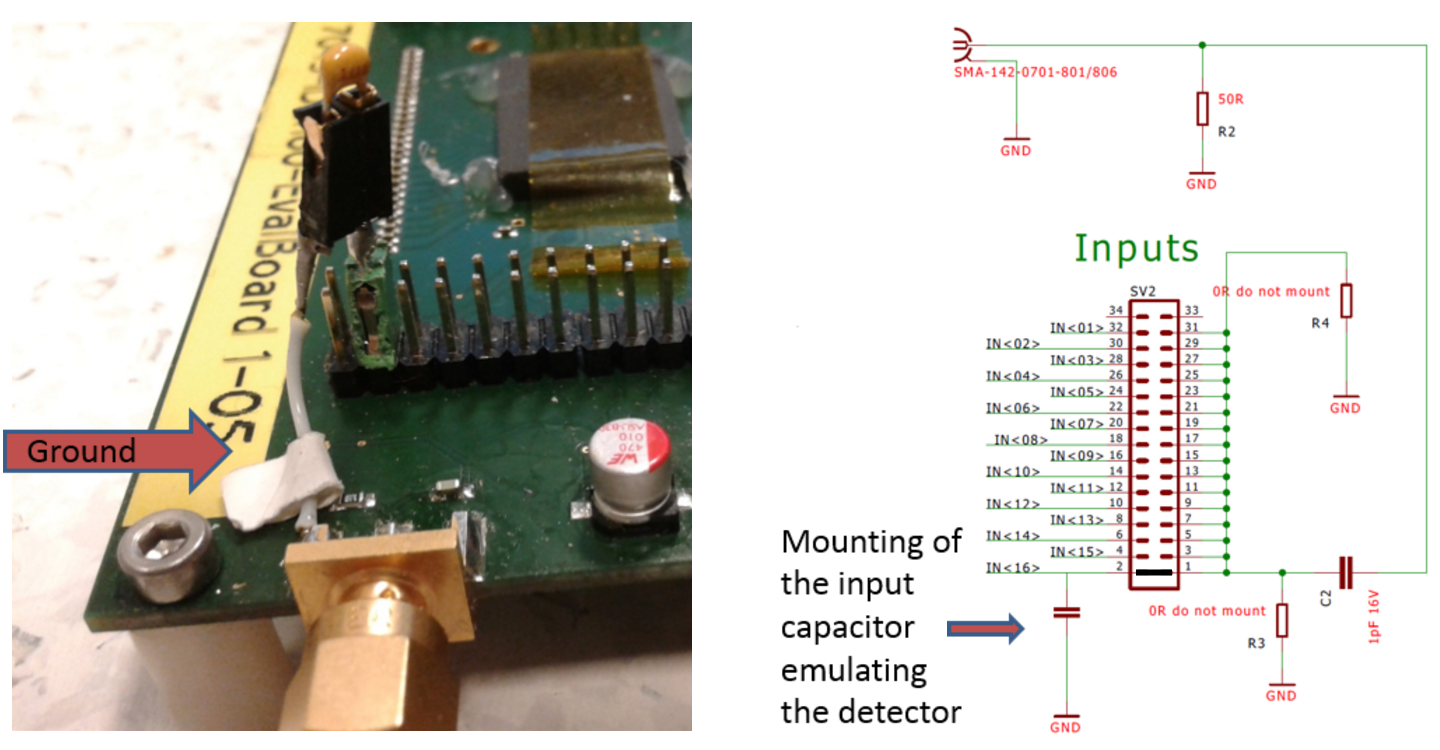
\includegraphics[width=\textwidth]{capamount.png}
	\caption{Image and schematic of capacitor mount. \citep{Thomas} \citep{IDE1180sch}}
	\label{fig-capmount}
\end{figure} 

The IDE1180 has been configured to six different shaping times: 40~ns (default), 100~ns, 300~ns, 500~ns, 1~$\mu$s, and 2~$\mu$s. The 100~ns and 300~ns settings have only been used to investigate the relationship between noise and shaping time. Table \ref{tab-ide-shaping} shows the necessary parameters to configure the IDE1180 to these shaping times. 40 ns is the default shaping time, and therefore requires no jumpers. The voltages specify the potential that should be across the 10~$k\Omega$ resistor belonging to said signal, and can be measured when a GND jumper is in place. PZ\_ENABLE enables the pole-zero cancellation on 3V3. PZ\_BIAS\_HI to 3V3 switches to high range of pole-zero time constant (low pole-zero resistance). SH\_BIAS adjusts the shaper operation current. VFS\_BIAS sets the peaking time. PZ\_BIAS adjusts the pole-zero time constant. SH\_BIAS and VFS\_BIAS must be enabled with 3V3 jumpers for settings to take effect, while for PZ\_BIAS settings take effect for a GND jumper. 

\begin{table}[h!]
	\centering
	\caption{Configurations for different shaping times on IDE1180.}
	\label{tab-ide-shaping}
	\makebox[\textwidth][c]{	%Center too large table
	\begin{tabular}{cccccc}\toprule
		\textbf{Shaping time} & \textbf{PZ\_ENABLE} & \textbf{PZ\_BIAS\_HI} & \textbf{SH\_BIAS}  & \textbf{VFS\_BIAS} & \textbf{PZ\_BIAS}    \\ \midrule
		40 ns        & X or GND          & X or GND            & X or GND        & X or GND        & X or GND          \\
		100 ns       & 3V3          & X or GND            & 3V3, 144 mV & 3V3, 132 mV  & GND, 110 mV   \\
		300 ns       & 3V3          & 3V3            & 3V3, 308 mV & 3V3, 81 mV  & GND, 1790 mV   \\
		500 ns       & 3V3          & 3V3            & 3V3, 325 mV & 3V3, 81 mV  & GND, 500 mV   \\
		1 $\mu$s     & 3V3          & 3V3            & 3V3, 350 mV & 3V3, 92 mV  & GND, 268 mV   \\
		2 $\mu$s     & 3V3          & 3V3            & 3V3, 357 mV & 3V3, 91 mV  & GND, 109.5 mV \\ \bottomrule
	\end{tabular}
	}
\end{table}


\section{Gain vs. Input Load Capacitance}
\label{ide-gain}

During early measurements it quickly became evident that the output voltage from the IDE1180 is reduced when the input load capacitance is increased, see figure \ref{fig-gain-drop}. This drop was at first not understood by the team. It was found to be caused by multiple effects, which are investigated in this section. Tables \ref{tab-gain-nobuffer} to \ref{tab-gain-nobuffer-offset} show gain measurements with different gain settings, using different setups. The oscilloscope measurements were done by placing a cursor in the middle of the noise using the Tektronix oscilloscope. The ADC measurements are calculated from the mean of a gaussian fit to amplitude measurements done by the ADC. The measurements shown in these tables were done with an input ramp pulse with 1~$\mu$s period from the Agilent oscilloscope.
%A "1" is either a jumper to the left, or no jumper at all, while a "0" is a jumper to the right. "11" is equal to default setting with no jumpers in place. 

\begin{figure}%[h]
	\centering
	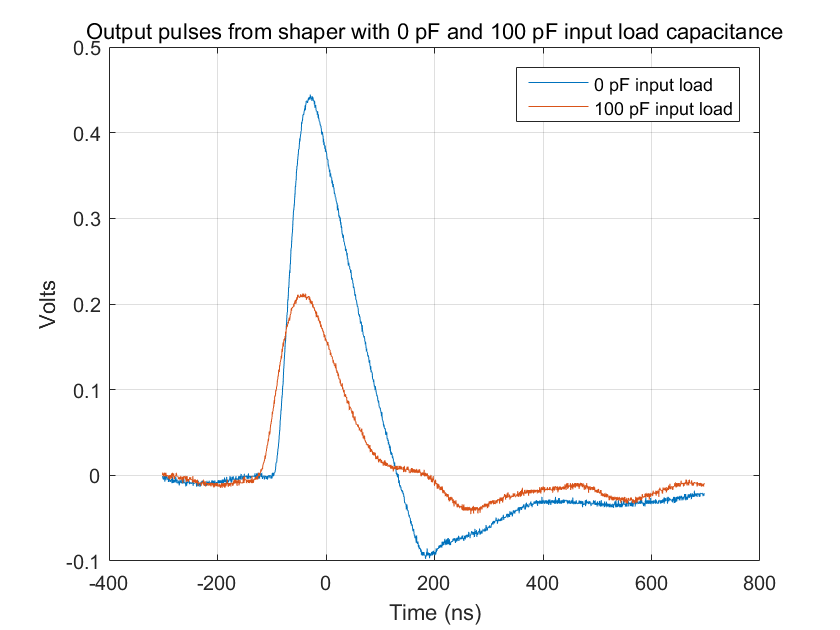
\includegraphics[width=0.6\textwidth]{shaper_pulses.png}
	\caption{Pulses from IDE1180 with different input load capacitance.}
	\label{fig-gain-drop}
\end{figure} 

\begin{table}[h!] %%XXX like this or not?
	\begin{center}
		\caption{Gain [mV/fC] vs. capacitance for different gain settings measured with oscilloscope without buffer connected.}
		\label{tab-gain-nobuffer}
		\begin{tabular}{clcccc}\toprule
			&\textbf{PA\_GAIN<1:0>} & \textbf{0pF}  & \textbf{10pF} & \textbf{56pF} & \textbf{100pF} \\ \midrule
%			"GND-GND"     & 11.4 & 10.1 & 6.6  & 5.1   \\
%			"GND-3V3"     & 7.0    & 6.3  & 4.6  & 3.8   \\
%			"3V3-GND"     & 4.3  & 4.1  & 3.4  & 3.0     \\
%			"3V3-3V3"     & 2.3  & 2.2  & 2.0    & 1.76 \\ \bottomrule
			00&GND-GND     & 11.2 & 9.9 & 6.5  & 5.0   \\
			01&GND-3V3     & 6.9    & 6.2  & 4.5  & 3.7   \\
			10&3V3-GND     & 4.2  & 4.0  & 3.3  & 2.9     \\
			11&3V3-3V3     & 2.3  & 2.2  & 2.0    & 1.7 \\ \bottomrule
		\end{tabular}
	\end{center}
\end{table}

\begin{table}[h!]
	\begin{center}
		\caption{Gain [mV/fC] vs. capacitance for different gain settings measured with oscilloscope with buffer connected.}
		\label{tab-gain-wbuffer}
		\begin{tabular}{clcccc}\toprule
			&\textbf{PA\_GAIN<1:0>} & \textbf{0pF}  & \textbf{10pF} & \textbf{56pF} & \textbf{100pF} \\ \midrule
%			"GND-GND"     & 10.2 & 8.6  & 5.4  & 4.3   \\
%			"GND-3V3"     & 6.0    & 5.4  & 4.0    & 3.2   \\
%			"3V3-GND"     & 3.6  & 3.5  & 2.9  & 2.5   \\
%			"3V3-3V3"     & 2.0    & 1.9  & 1.6  & 1.4 \\ \bottomrule
			00&GND-GND     & 10.0 & 8.4  & 5.3  & 4.2   \\
			01&GND-3V3    & 5.9    & 5.3  & 3.9    & 3.1   \\
			10&3V3-GND     & 3.5  & 3.4  & 2.8  & 2.5   \\
			11&3V3-3V3     & 2.0    & 1.9  & 1.6  & 1.4 \\ \bottomrule
		\end{tabular}
	\end{center}
\end{table}


\begin{table}[h!]
	\begin{center}
		\caption{Gain [mV/fC] vs. capacitance measured with ADC.}
		\label{tab-gain-adc}
		\begin{tabular}{clcccc}\toprule
			&\textbf{PA\_GAIN<1:0>} & \textbf{0pF}  & \textbf{10pF} & \textbf{56pF} & \textbf{100pF} \\ \midrule
%			"GND-GND"     & 10.8 & 9.4  & 5.8  & 4.5   \\ \bottomrule
			00 &GND-GND     & 10.6 & 9.2  & 5.7  & 4.4   \\ \bottomrule
		\end{tabular}
	\end{center}
\end{table}

\begin{table}[h!]
	\begin{center}
		\caption{Gain [mV/fC] vs. capacitance for different gain settings measured with oscilloscope without buffer connected. Input load capacitor connected to $V_{offset}$ instead of ground.}
		\label{tab-gain-nobuffer-offset}
		\begin{tabular}{clccc}\toprule
			&\textbf{PA\_GAIN<1:0>} & \textbf{0pF}  & \textbf{56pF} & \textbf{100pF} \\ \midrule
%			"GND-GND"     & 10.2 & 5.8  & 4.44  \\
%			"GND-3V3"     & 6.3  & 4.1  & 3.5   \\
%			"3V3-GND"     & 3.75 & 2.95 & 2.6   \\
%			"3V3-3V3"     & 2.05 & 1.75 & 1.5   \\ \bottomrule
			00&GND-GND     & 10.7 & 6.1  & 4.6  \\
			01&GND-3V3     & 6.6  & 4.3  & 3.7   \\
			10&3V3-GND     & 3.9 & 3.1 & 2.7   \\
			11&3V3-3V3     & 2.2 & 1.8 & 1.6   \\ \bottomrule
		\end{tabular}
	\end{center}
\end{table}

As the ADC measurements takes the maximum peak signal, while the oscilloscope measurements are done with cursors in the center of the peak noise, it was expected that the table \ref{tab-gain-adc} values were slightly higher than the table \ref{tab-gain-wbuffer} values. The values in table \ref{tab-gain-wbuffer} are 10 to 20 \% lower than those in table \ref{tab-gain-nobuffer}, showing that the in-house buffer does not perfectly pass the signal. This could be caused by gain lower than one, bandwidth limitations, or impedance problems. It should also be noted that the measured gains at 0 pF are very different from the gains of 24/12/6/3 mV/fC that are noted in the datasheet \citep{IDE1180}. \comm{ The values in table \ref{tab-gain-nobuffer-offset} are 8 to 15 \% lower than those in table \ref{tab-gain-nobuffer}.}



Figure \ref{fig-IDE1180-gain} shows how the gain falls off for the different shaping times. This is measured using the Agilent oscilloscope, with the IDE1180 inside a Faraday cage. The drop becomes less and less distinct as the shaping time is increased, and at 2~$\mu$s the gain vs. capacitance curve is fairly flat. It is possible to increase the gain of the IDE1180 by 50~\% with the BUF\_GAIN\_HI setting. This can for example be useful when using the IDE1180 with long shaping times where the gain is very low.

\subsubsection{Faraday cage load issue}
Note that the default shaping time curve in figure \ref{fig-IDE1180-gain} does not fit well with the data in the tables in this section. This was first assumed to be due to the differences in the two 1~pF test capacitors and the imperfect gain of the buffer, but after the 1~pF was compensated for it became obvious that this was not the only contributor. The real main reason was very late discovered to be the line capacitance of the Faraday cage and the cables on the output, see figure \ref{fig-box-pulse}. The IDE1180 is made to drive a line capacitance of nominally 4~pF and maximum 20~pF \citep{IDE1180}. The extra capacitance from the box and extra cables causes the pulse height to drop and the pulse fall time to increase. It was attempted to counter this by tuning the BUF\_BIAS input, which is the output buffer operation current, but this only caused the opposite effect by increasing the fall time and reducing the peak height. 
%% 1pF replaced blah blah

%% teste om forskjell på gain skyldes dc block før/etter buffer. Eller annen signalgenerator. kanskje fordi 1pf ble byttet ut (29.04)....

\begin{figure}%2016.07.18
	\centering
	\begin{subfigure}{.5\textwidth}
		\centering
		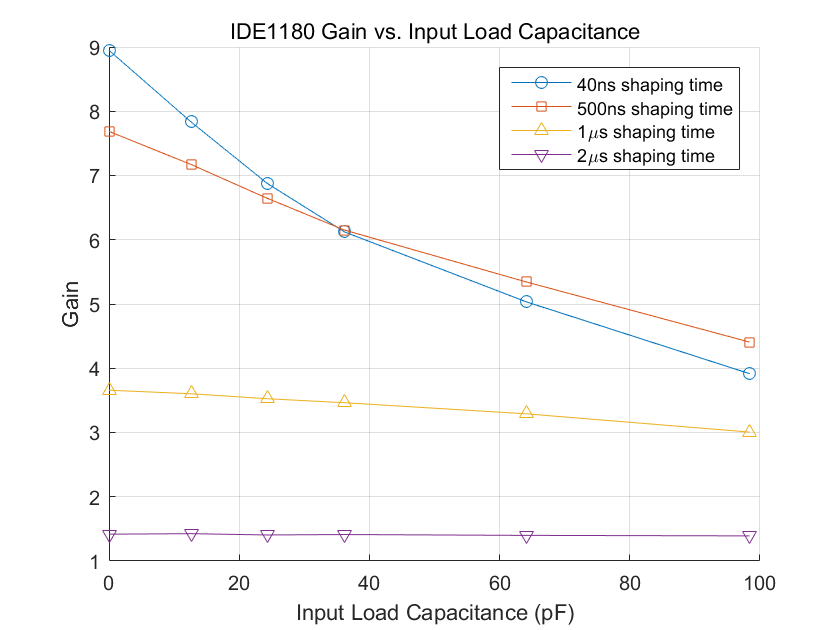
\includegraphics[width=\linewidth]{Gain_shaping.png}
		\caption{Gain.}
		\label{fig-IDE1180-gain-}
	\end{subfigure}%
	\begin{subfigure}{.5\textwidth}
		\centering
		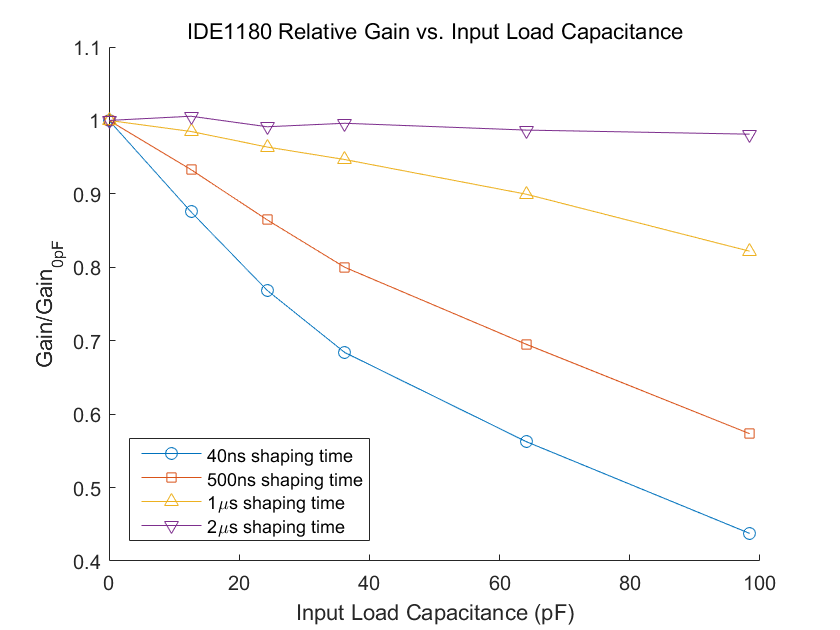
\includegraphics[width=\textwidth]{Gain_shaping_relative.png}
		\caption{Relative gain.}
		\label{fig-IDE1180-gain-rel} %need to check permission
	\end{subfigure}
	\caption{Gain and relative gain vs. capacitance at different shaping times.}
	\label{fig-IDE1180-gain}
\end{figure}

\begin{figure}%[h]
	\centering
	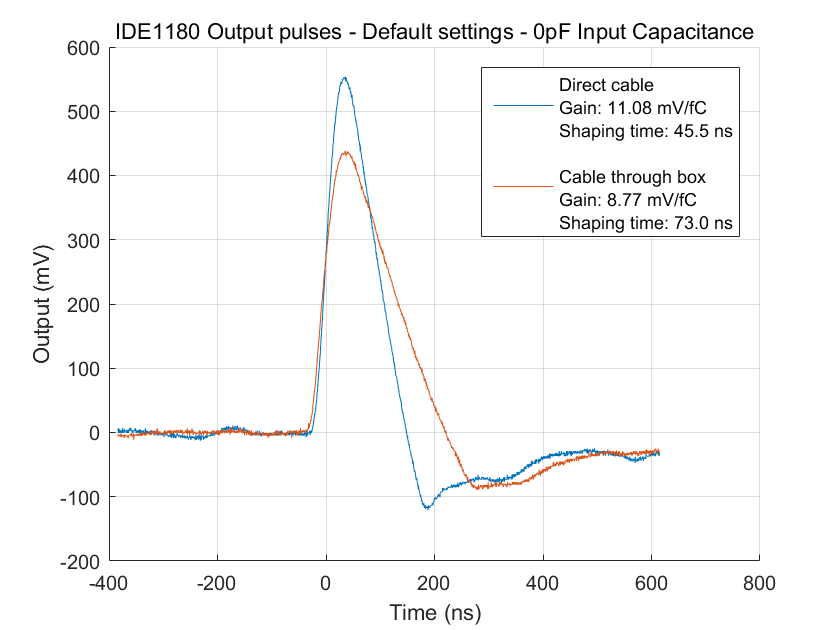
\includegraphics[width=0.6\textwidth]{boxpulse.png}
	\caption{Pulses from IDE1180 with (blue) a direct cable from IDE1180 to Agilent oscilloscope, and (red) with first a cable to a connector on the Faraday cage and a cable on the other side to the oscilloscope.}
	\label{fig-box-pulse}
\end{figure} 

\subsection{Gain vs. Capacitance Simulations}

To investigate the behaviour of a pre-amplifier being loaded with an input capacitance, a pre-amplifier was simulated in LTspice IV. One of the pre-amplifiers from \citep{tali} was simulated (figure \ref{fig-sim-sch}), as the specifications of the IDE1180 pre-amplifier are unavailable. This was simulated both with an ideal \gls{opamp}, and with the LT1122 that was tested in \citep{tali}. LT1122 is a fast settling amplifier with a good bandwidth, but is noisy and was therefore not used for the pre-amplifier in Tali's final design. The input signal for this simulation was a square wave of 2 ms period, 100 mV amplitude, and 10 ns edge times. Simulations were performed for $C_{load}$ of 1 pF and 100 pF.  

\begin{figure}
\centering
\begin{circuitikz}  
	\draw  
	(5,2) node[op amp] (opamp) {}  
	(0,2.5) to [C, l=$1 pF$] (opamp.-)
	(3,0.5)  to [C=$C_{load}$] (3,2.5)
	(0,2.5) to [short, -] (0,2.5)  
	(0,0.5) to [short, -o] (7,0.5)  
	(3.8,0.5) to [short, -] (opamp.+)  
	(3.8,3.5) to [R, l=$4.7 M\Omega$] (6.2,3.5) 
	(3.8,5) to [C, l=$2.2 pF$] (6.2,5) 
	(3.8,5) to [short, -] (opamp.-)  
	(6.2,5) to [short, -] (opamp.out)  
	(opamp.out) to [short, -o] (7, 2)  
	(0,2.5) to[sqV,v=$V_{in}$] (0,0.5);
	\draw[->] 
	(6.75,1.8) to node[right] {$V_{out}$} (6.75,0.7);
\end{circuitikz}
\caption{Schematic of simulated circuit.}
\label{fig-sim-sch}
\end{figure}

\begin{figure}%[h]
	\centering
	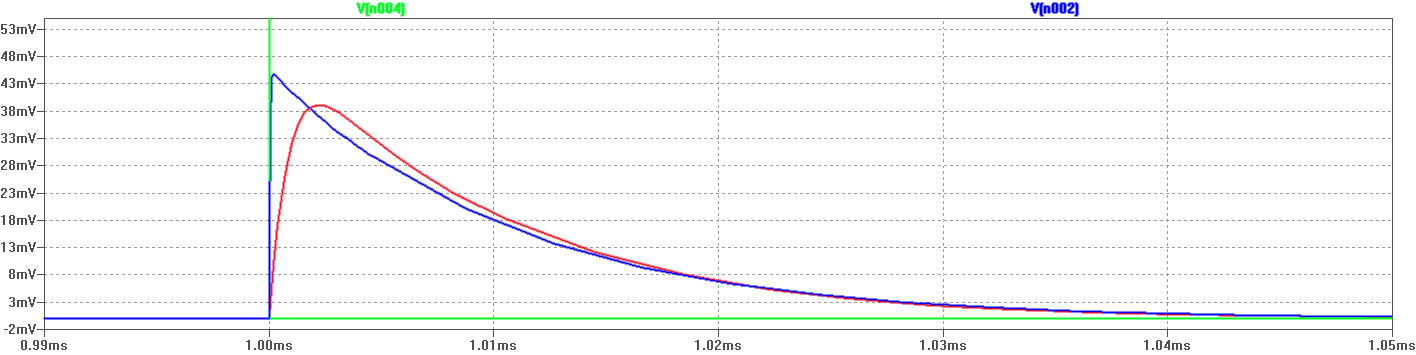
\includegraphics[width=\textwidth]{sim_ideal_both.png}
	\caption{Simulation of ideal \gls{opamp} with 1 pF (blue) and 100 pF (red) load capacitance. Input pulse in green.}
	\label{fig-sim-ideal}
\end{figure} 

\begin{figure}%[h]
	\centering
	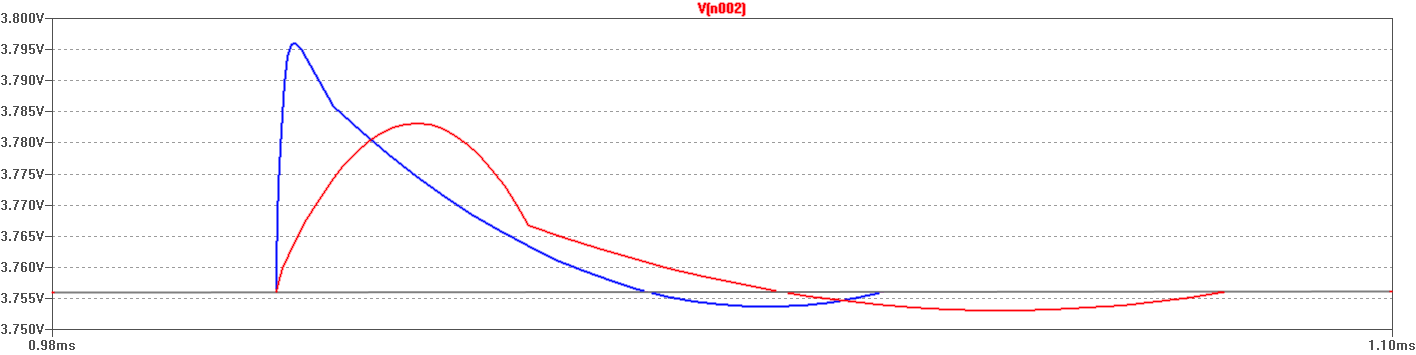
\includegraphics[width=\textwidth]{sim_LT1122_both.png}
	\caption{Simulation of LT1122 \gls{opamp} with 1 pF (blue) and 100 pF (red) load capacitance.}
	\label{fig-sim-LT1122}
\end{figure} 

For the ideal \gls{opamp}, figure \ref{fig-sim-ideal} shows a peak height drop of roughly 9 \% and an increase in pulse area of about 1 \% when the load capacitance is increased from 1 pF to 100 pF. Similarly for the LT1122, figure \ref{fig-sim-LT1122} shows a peak height drop of about 32 \% and a pulse area increase of roughly 11 \%. Compared to the measured peak amplitude drops of almost 60 \%, this shows that the drops should have been expected, but not in that magnitude. This has later been confirmed by figure \ref{fig-ide-gain} which shows an expected peak amplitude drop of about 10 \% at 100 pF, calculated by IDEAS. 
%For the ideal \gls{opamp}, figure \ref{fig-sim-ideal} shows a peak height drop of roughly 9 \% and an increase in pulse area of about 1 \% when the load capacitance is increased from 1 pF to 100 pF. Similarly for the LT1122, figure \ref{fig-sim-LT1122} shows a peak height drop of about 32 \% and a pulse area increase of roughly 11 \%. Calculations by IDEAS, figure \ref{fig-ide-gain}, shows an expected peak amplitude drop of about 10 \% at 100 pF. Compared to the measured peak amplitude drops of almost 60 \%, these graphs show that the drops should have been expected, but not in that magnitude. 

XXX discuss lt1122 shape

\begin{figure}%[h]
	\centering
	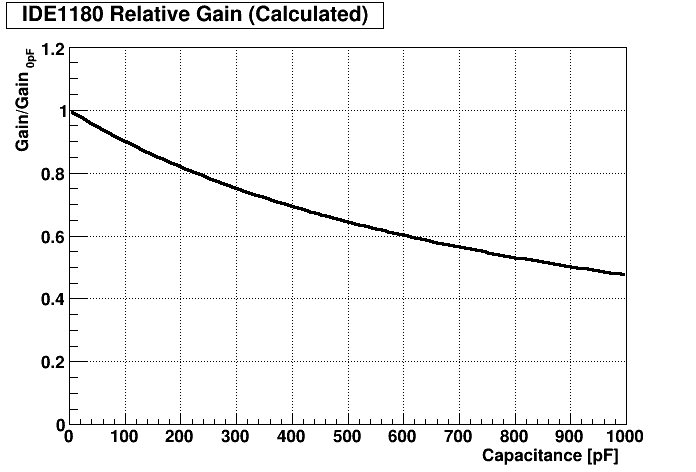
\includegraphics[width=0.6\textwidth]{IDE1180-gain.png}
	\caption{Calculated change in gain from increased input load capacitance. \citep{IDE1180email}}
	\label{fig-ide-gain}
\end{figure} 

One possible explanation for the gain drop could be leakage current from the capacitor. Since a large capacitance causes the rise time of the pulse to be very slow, it is possible that the leakage causes the pulse never being able to reach proper maximum value. 

\subsection{Ballistic deficit}
\label{ide-gain-ballistic}
%http://ns.ph.liv.ac.uk/~ajb/radiometrics/glossary/ballistic_deficit.html
%http://ns.ph.liv.ac.uk/~ajb/radiometrics/practical_analysis/practical_aspects/shaping_time_constant.htm
%http://www-physics.lbl.gov/~spieler/USPAS-MSU_2012/pdf/IV_Signal_Processing.pdf

Ballistic deficit (see section \ref{t-shaper}) is an error source that was investigated as a contributor to the drop in amplitude for high load capacitors.\comm{ This occurs when a too short shaping time compared to the rise time of the input pulse leads to a decrease in amplitude. When the shaping time is too short, not all of the charge will have had time to be collected, and the output pulse does not reach the full amplitude.} Figures \ref{fig-IDE1180-shaperamp} to \ref{fig-IDE1180-shaperrisetime} show measurements investigating the drop in gain by comparing the output signal from the IDE1180 when the shaper is connected and disconnected using the SH\_ENABLE pin header. This is measured at default settings, using the Agilent oscilloscope, and the IDE1180 inside a Faraday cage. These data are based on only one curve saved from the oscilloscope, except  for 100 pF with shaper disabled, where two curves were saved as the signal was very noisy. Therefore this data is not very accurate, but it is good for observing trends. 

%2016.06.21
\begin{figure}[p]
	\centering
	\begin{subfigure}{.5\textwidth}
		\centering
		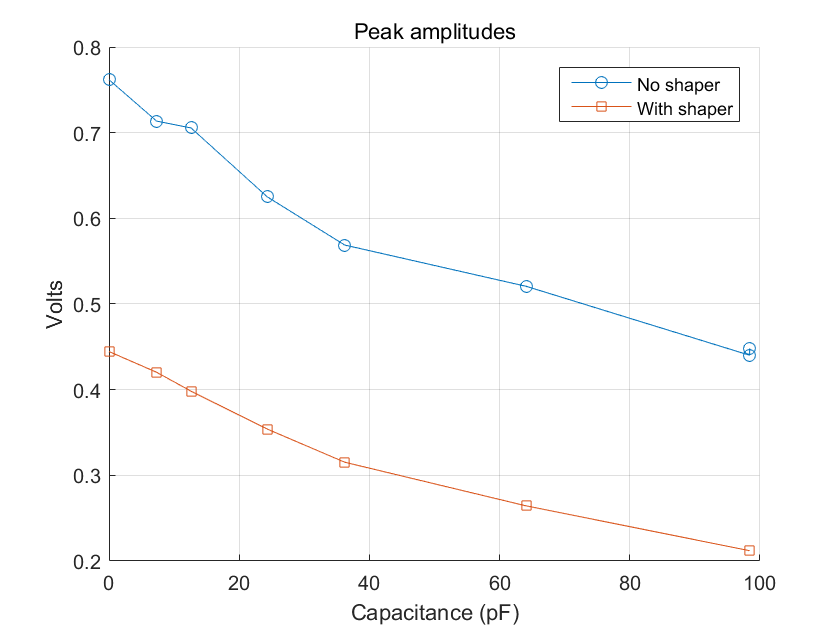
\includegraphics[width=\linewidth]{shaper_amplitude.png}
		\caption{Peak amplitudes.}
		\label{fig-IDE1180-shaperamp-}
	\end{subfigure}%
	\begin{subfigure}{.5\textwidth}
		\centering
		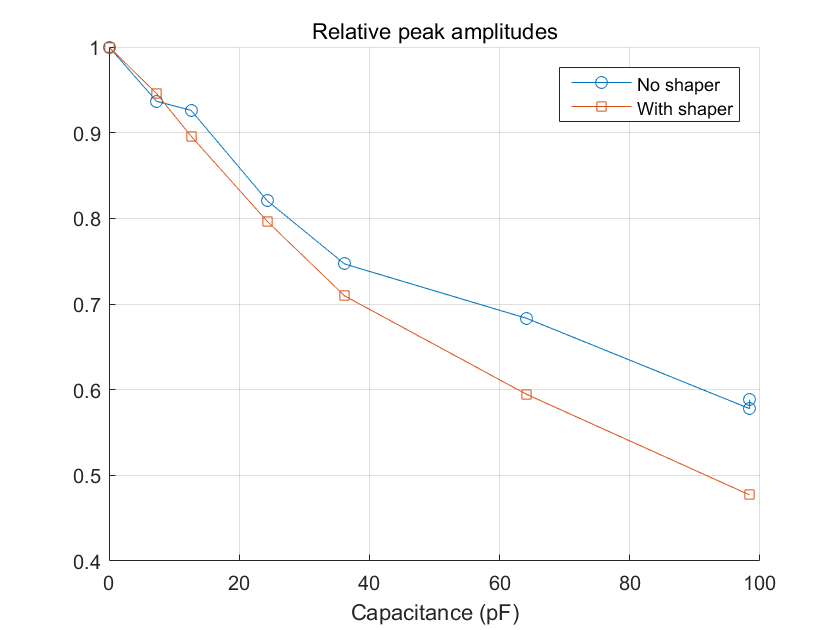
\includegraphics[width=\textwidth]{shaper_amplitude_relative.png}
		\caption{Relative peak amplitudes.}
		\label{fig-IDE1180-shaperamp-rel} 
	\end{subfigure}
	\caption{Amplitude comparison with and without shaper connected.}
	\label{fig-IDE1180-shaperamp}
\end{figure}

\begin{figure}[p]
	\centering
	\begin{subfigure}{.5\textwidth}
		\centering
		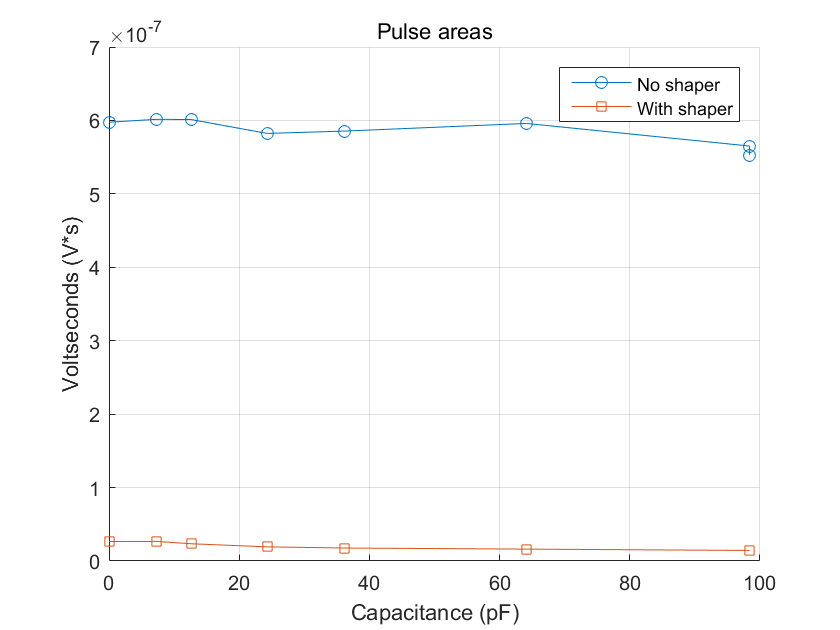
\includegraphics[width=\linewidth]{shaper_area.png}
		\caption{Pulse areas.}
		\label{fig-IDE1180-shaperarea-}
	\end{subfigure}%
	\begin{subfigure}{.5\textwidth}
		\centering
		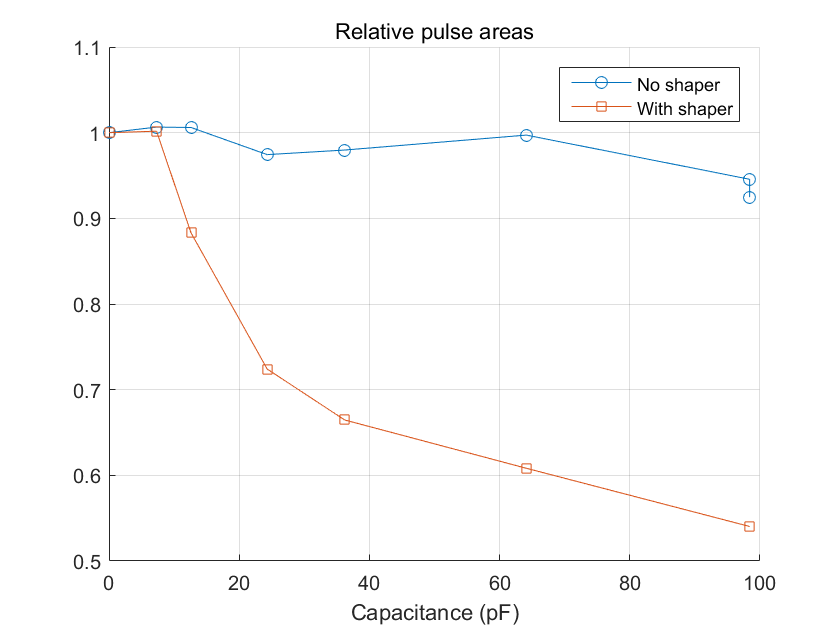
\includegraphics[width=\textwidth]{shaper_area_relative.png}
		\caption{Relative pulse areas.}
		\label{fig-IDE1180-shaperarea-rel} 
	\end{subfigure}
	\caption{Area comparison with and without shaper connected.}
	\label{fig-IDE1180-shaperarea}
\end{figure}

\begin{figure}[p]
	\centering
	\begin{subfigure}{.5\textwidth}
		\centering
		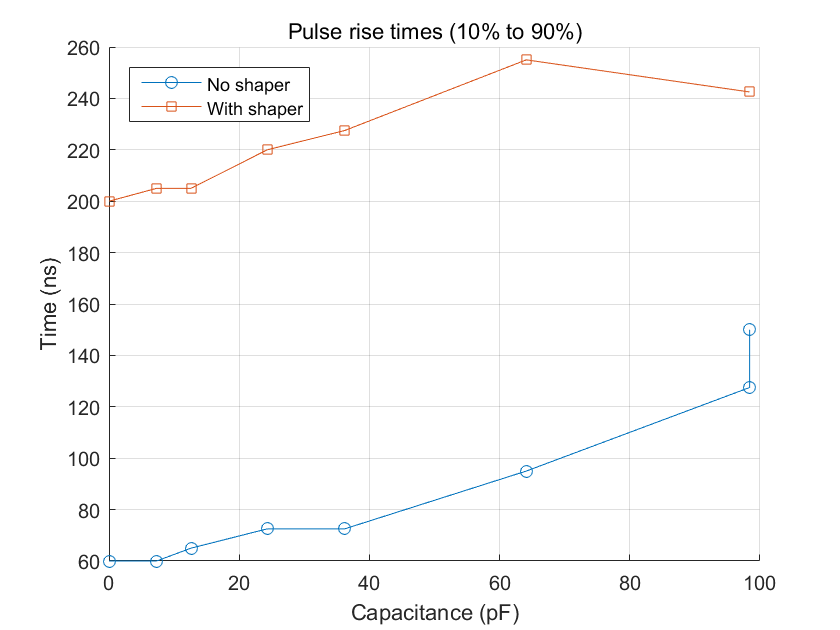
\includegraphics[width=\linewidth]{shaper_risetime.png}
		\caption{Pulse peaking times.}
		\label{fig-IDE1180-shaperrisetime-}
	\end{subfigure}%
	\begin{subfigure}{.5\textwidth}
		\centering
		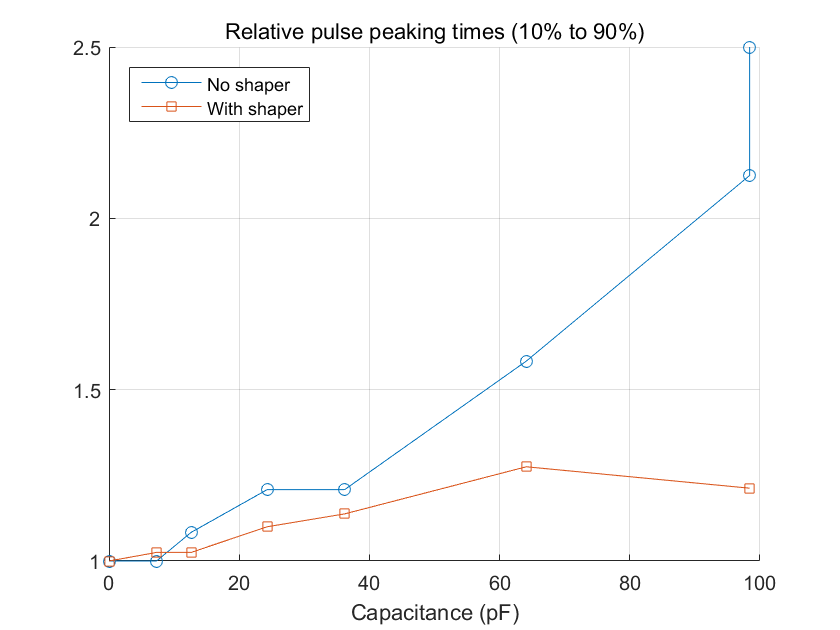
\includegraphics[width=\textwidth]{shaper_risetime_relative.png}
		\caption{Relative pulse peaking times.}
		\label{fig-IDE1180-shaperrisetime-rel}
	\end{subfigure}
	\caption{Pulse peaking time comparison with and without shaper connected.}
	\label{fig-IDE1180-shaperrisetime}
\end{figure}

%Figure \ref{fig-IDE1180-shaperamp-rel} shows that the shaper contributes only a minor part of the gain reduction. 
In figure \ref{fig-IDE1180-shaperrisetime-} we see that even at 0 pF input load capacitance, the peaking time of the pulse from the pre-amplifier is 60 ns, which is longer than the shaping time of 40 ns. As the capacitance is increased, the peaking time is greatly increased, and we see the difference between the two curves in figure \ref{fig-IDE1180-shaperamp-rel} increasing. This appears to be a ballistic deficit, but as gain reduction in the shaper from the increased capacitance is only about one fifth of the total gain reduction, ballistic deficit does not seem to be the main issue.  

%\subsection{PCB Input Capacitance}
%\label{ide-gain-pcb}
%Higher than expected
%Slope of sim is so much lower, so probably not this. 

\newpage
\section{Noise Measurements}
\label{ide-noise}

Noise measurements on the IDE1180 have been performed with the ADC setup in figure \ref{fig-setup-adc}, and the IDE1180 inside a Faraday cage. Three different methods have been used to measure the noise:
\begin{enumerate}  
	\item No input signal. Fit a Gaussian to the raw signal histogram. 
	\item With pulse on input. Fit a Gaussian to the raw signal histogram.  
	\item With pulse on input. Using peak detection. Fit a Gaussian to the peak histogram.   
\end{enumerate}

The results were expected to be somehow different on method three as it does not use the same histogram. Methods one and two observe variations in the baseline, while method three observes variations in the peak height. Figure \ref{fig-noise-methods} shows a comparison of measurement results on the same system with the three different methods. All methods show a slightly different slope. For method two, the higher noise values at high capacitance is because the histogram consists of two overlapping Gaussians.  %If the noise varies between 10 mV and 30 mV, the raw signal measurements will see noise up to 30 mV, while the peak measurement will only see noise of 20 mV, because the period of the noise is much shorter than the peak width. 

\begin{figure}[h!]   %2016.04.18
	\centering
	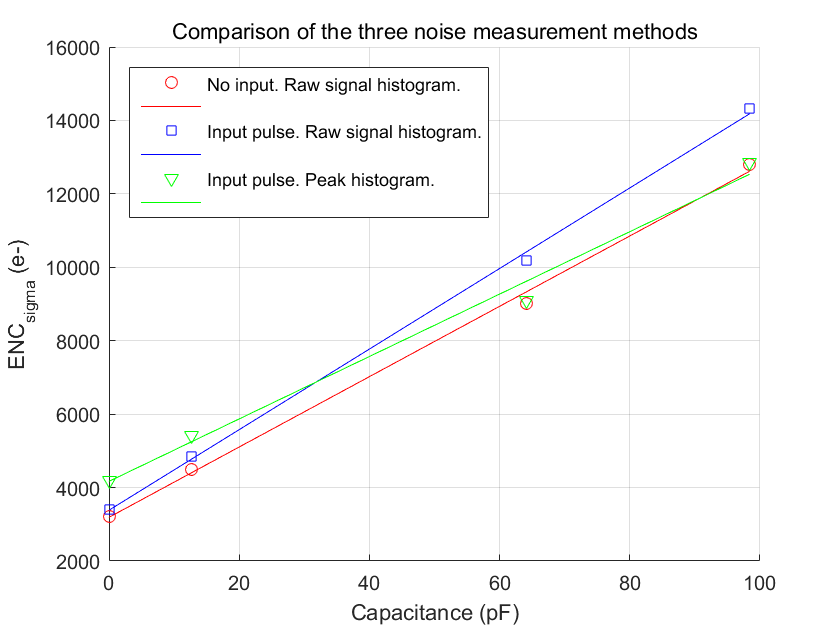
\includegraphics[width=0.7\textwidth]{Noise-methods.png}
	\caption{Comparison of the three noise measurement methods used.}
	\label{fig-noise-methods}
\end{figure} 

Noise is calculated as \acrfull{ENC}, the number of electrons needed on the input to create a signal equivalent to the measured noise, using eq. \ref{eq-noise}, where G is the gain, and $\sigma$ (sigma) is the standard deviation of the noise histogram. The noise can also be given in \gls{FWHM} by multiplying with $2\sqrt{2*ln2}$ ($\approx 2.355$). 

\begin{equation}%[h]
ENC_\sigma [e-] = \frac{\sigma [mV]}{G [mV/fC]*1.6*10^{-4} [fC/e-]}
\label{eq-noise}
\end{equation}

It is unknown if the noise measurement from IDEAS, figure \ref{fig-ide-noise}, is measured from the baseline variations or peak height variations, or if it is calculated as $\sigma$ or \gls{FWHM}. It is therefore hard to compare to this measurement. 

\begin{figure}%[h]
	\centering
	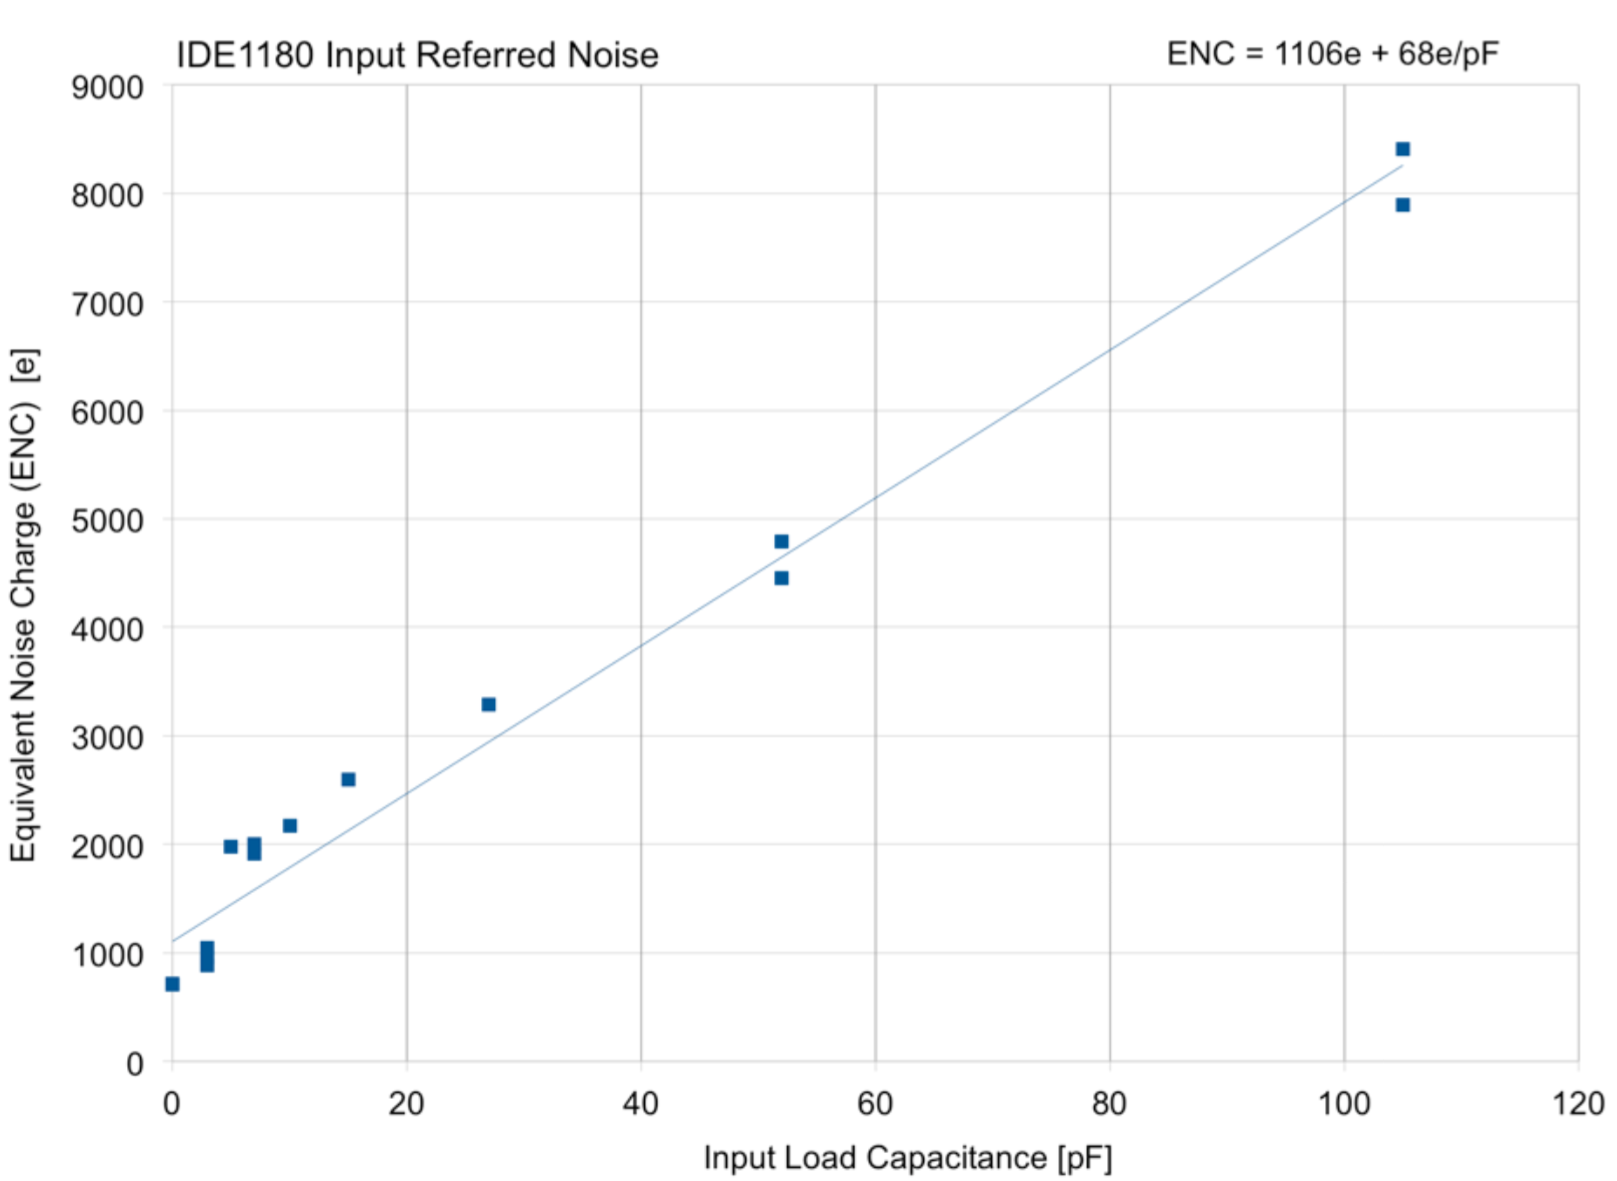
\includegraphics[width=0.7\textwidth]{IDE1180-noise.png}
	\caption{Measurement of the \gls{ENC} vs. input capacitive load. \citep{IDE1180}}
	\label{fig-ide-noise}
\end{figure} 

Figure \ref{fig-noise-nocomp} shows a noise measurement using method 3, calculated with a gain of 12~mV/fC, as specified in the datasheet \citep{IDE1180}. It is clear that the slope is extremely low, about 25~\%, compared to the measurement from IDEAS in figure \ref{fig-ide-noise}. 

\subsection{Gain Compensation}
\label{ide-noise-gain}

\begin{figure} 
	\centering
	\begin{subfigure}{.5\textwidth}
		\centering
		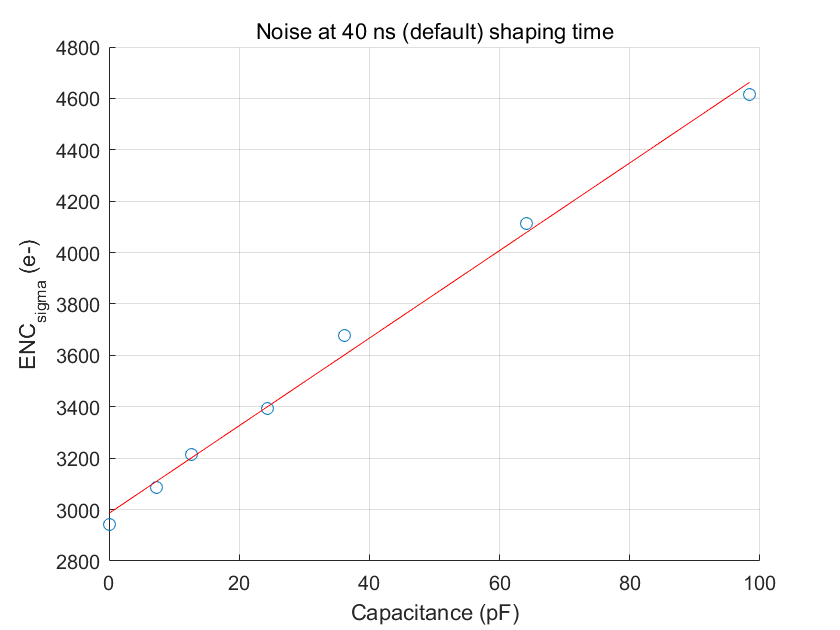
\includegraphics[width=\textwidth]{noise-default-nocomp.png}
		\caption{Calculated with gain of 12~mV/fC.}
		\label{fig-noise-nocomp}
	\end{subfigure}%
	\begin{subfigure}{.5\textwidth}%2016.06.22
		\centering
		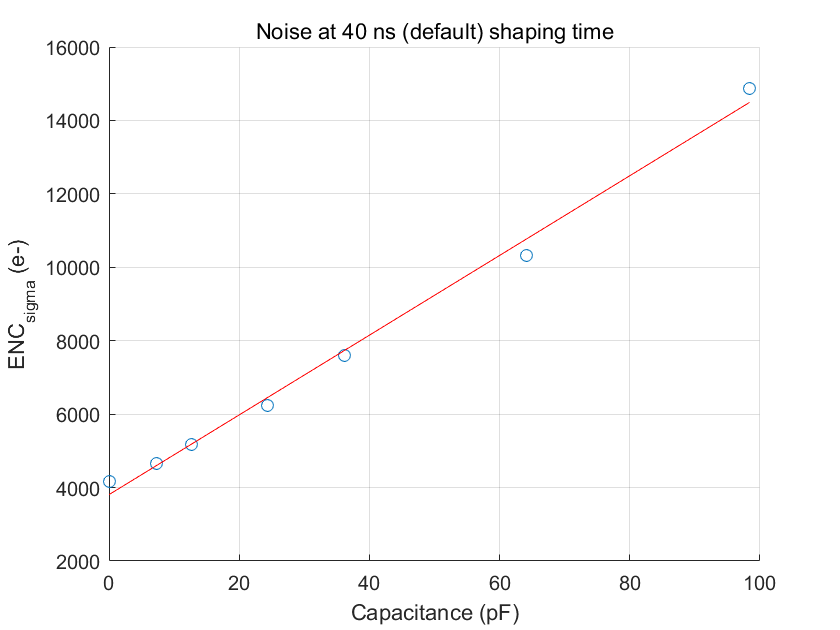
\includegraphics[width=\textwidth]{noise-default-auto.png}
		\caption{Calculated with automatic gain compensation.}
		\label{fig-noise-auto} 
	\end{subfigure}
	\caption{Measurements of the \gls{ENC} vs. input capacitive load. Calculated with constant and changing gain.}
	\label{fig-noise-nocomp-auto}
\end{figure}

As shown in equation \ref{eq-noise}, the gain is required to calculate the equivalent input noise, but as discussed in section \ref{ide-gain} the gain varies with input load capacitance. It is therefore necessary to change the gain for different capacitances in the noise calculation. Originally, this was done using the tables in section \ref{ide-gain}, but as this is not optimal in case something in the system is changed. Therefore the MATLAB script for plotting the gain was modified to also calculate the gain at each capacitance when the third method for noise measurements was used. The gain is simply calculated by taking the mean of the peak histogram and dividing by the input charge. 

When gain compensation is performed, see figure \ref{fig-noise-auto}, the noise curves have a slope very close to the one shown in the datasheet. Figure \ref{fig-noise-all} shows the noise curves for all configured shaping times. We see that for longer shaping times, the noise becomes much less dependant on the capacitance. Figure \ref{fig-noise-shape} shows how the noise changes with shaping time. Unlike figure \ref{fig-noise-min}, this does not show a single minimum. The absolute minimum is at 100 ns, but there is a local minimum at 1 $\mu$s, where the absolute minimum was expected to be from theory. This non-linear behaviour could be explained by that it is not only the shaping time constant that is being changed for the different shaping times, but also the pole-zero cancellation, which has a large impact on the noise. Figure \ref{fig-noise-all-output} shows the noise in mV measured on the output of the IDE1180. Here the two longest shaping times show the lowest noise levels, but since the gain is very low at these shaping times, the equivalent input noise is still high. 

\begin{figure}[p] %Noise combine
	\centering
	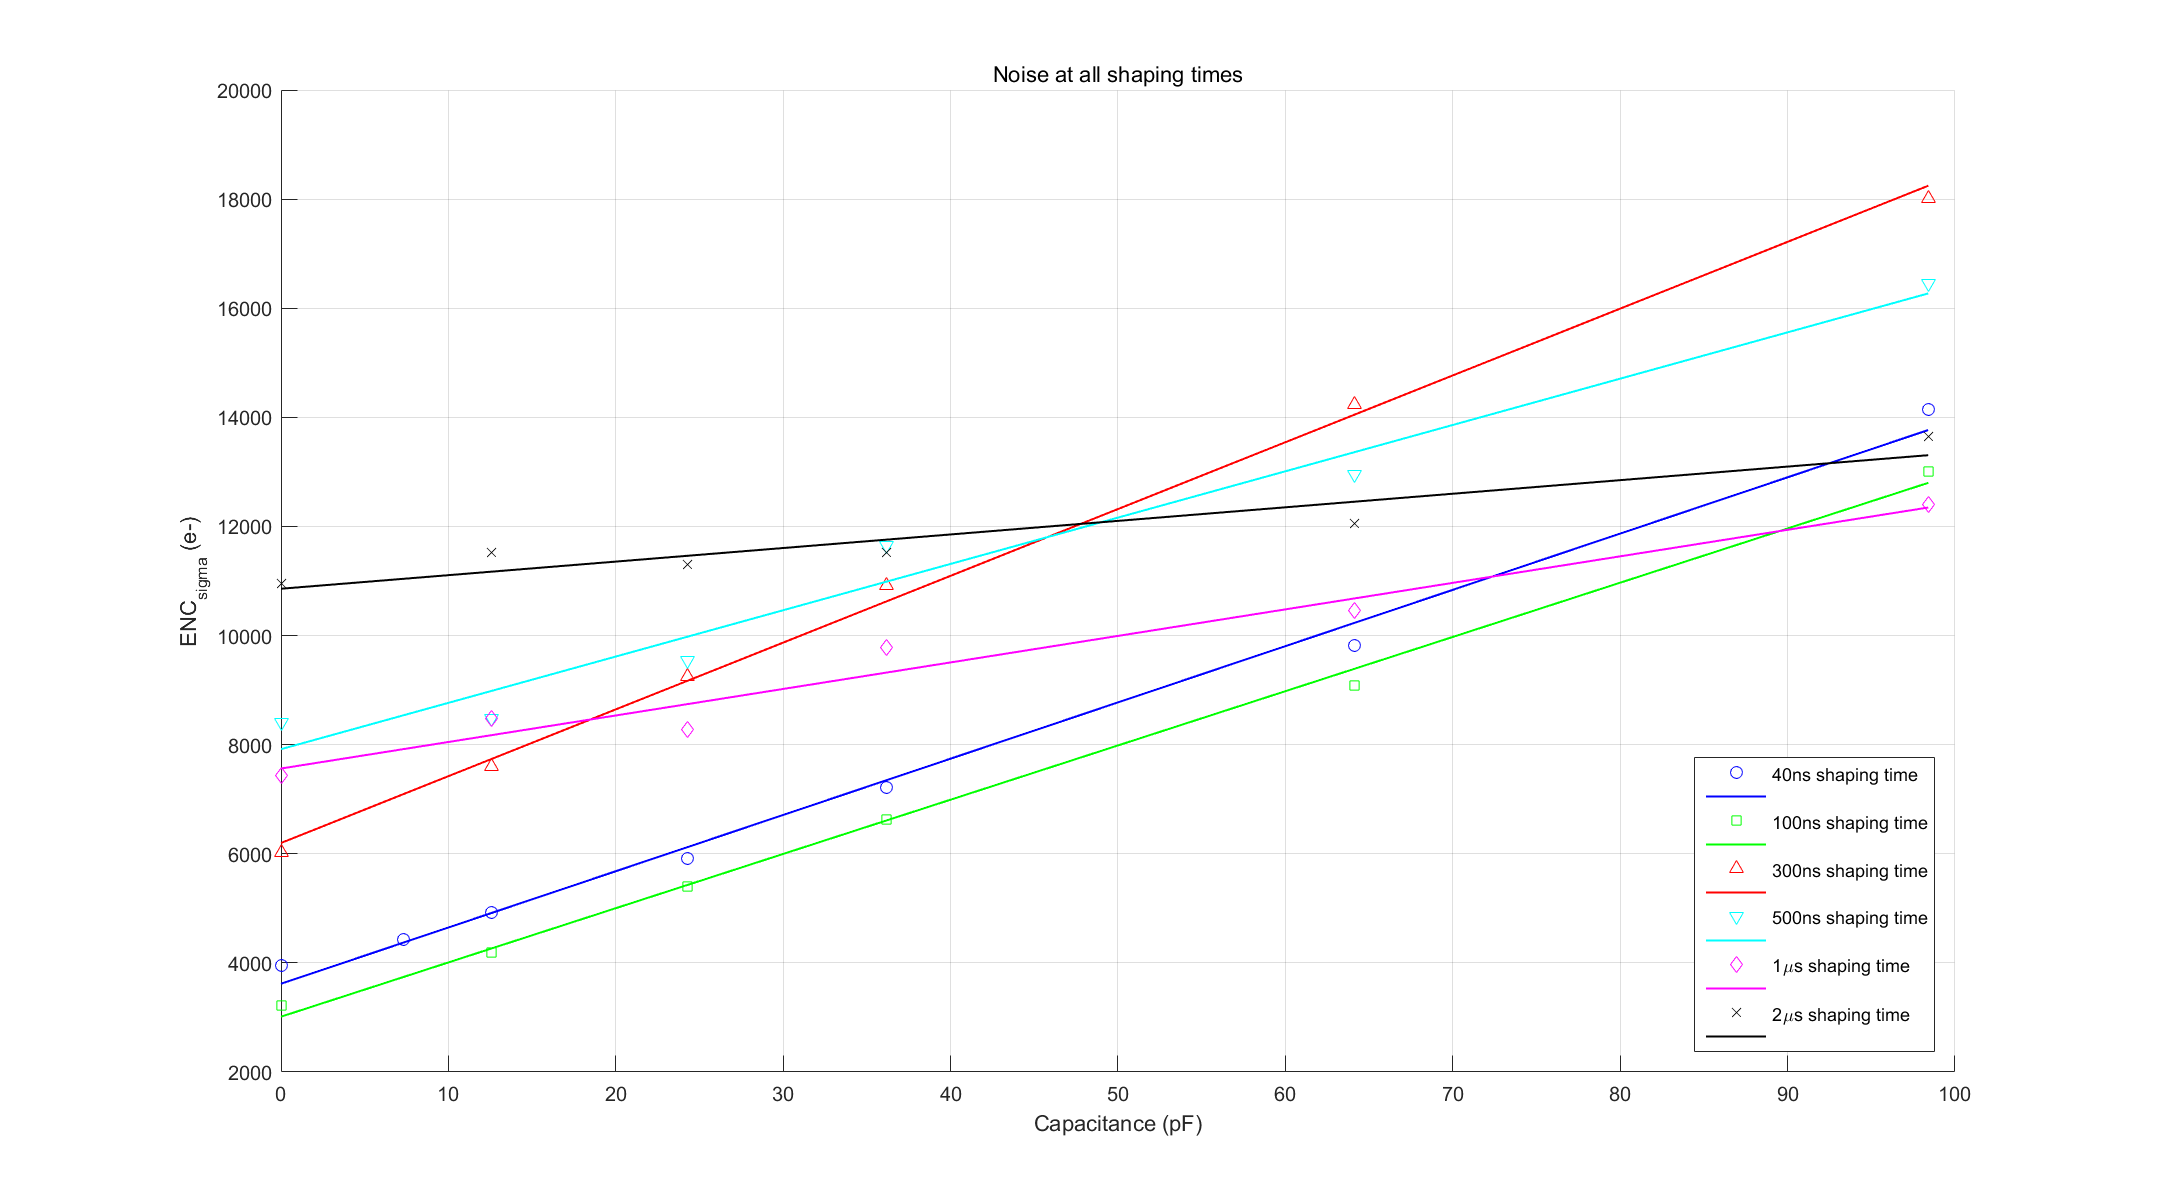
\includegraphics[width=\textwidth]{noise-all.png}
	\caption{Measurements of the \gls{ENC} vs. input capacitive load. Calculated with automatic gain compensation.}
	\label{fig-noise-all}
\end{figure} 

\begin{figure}[p] %Noise combine
	\centering
	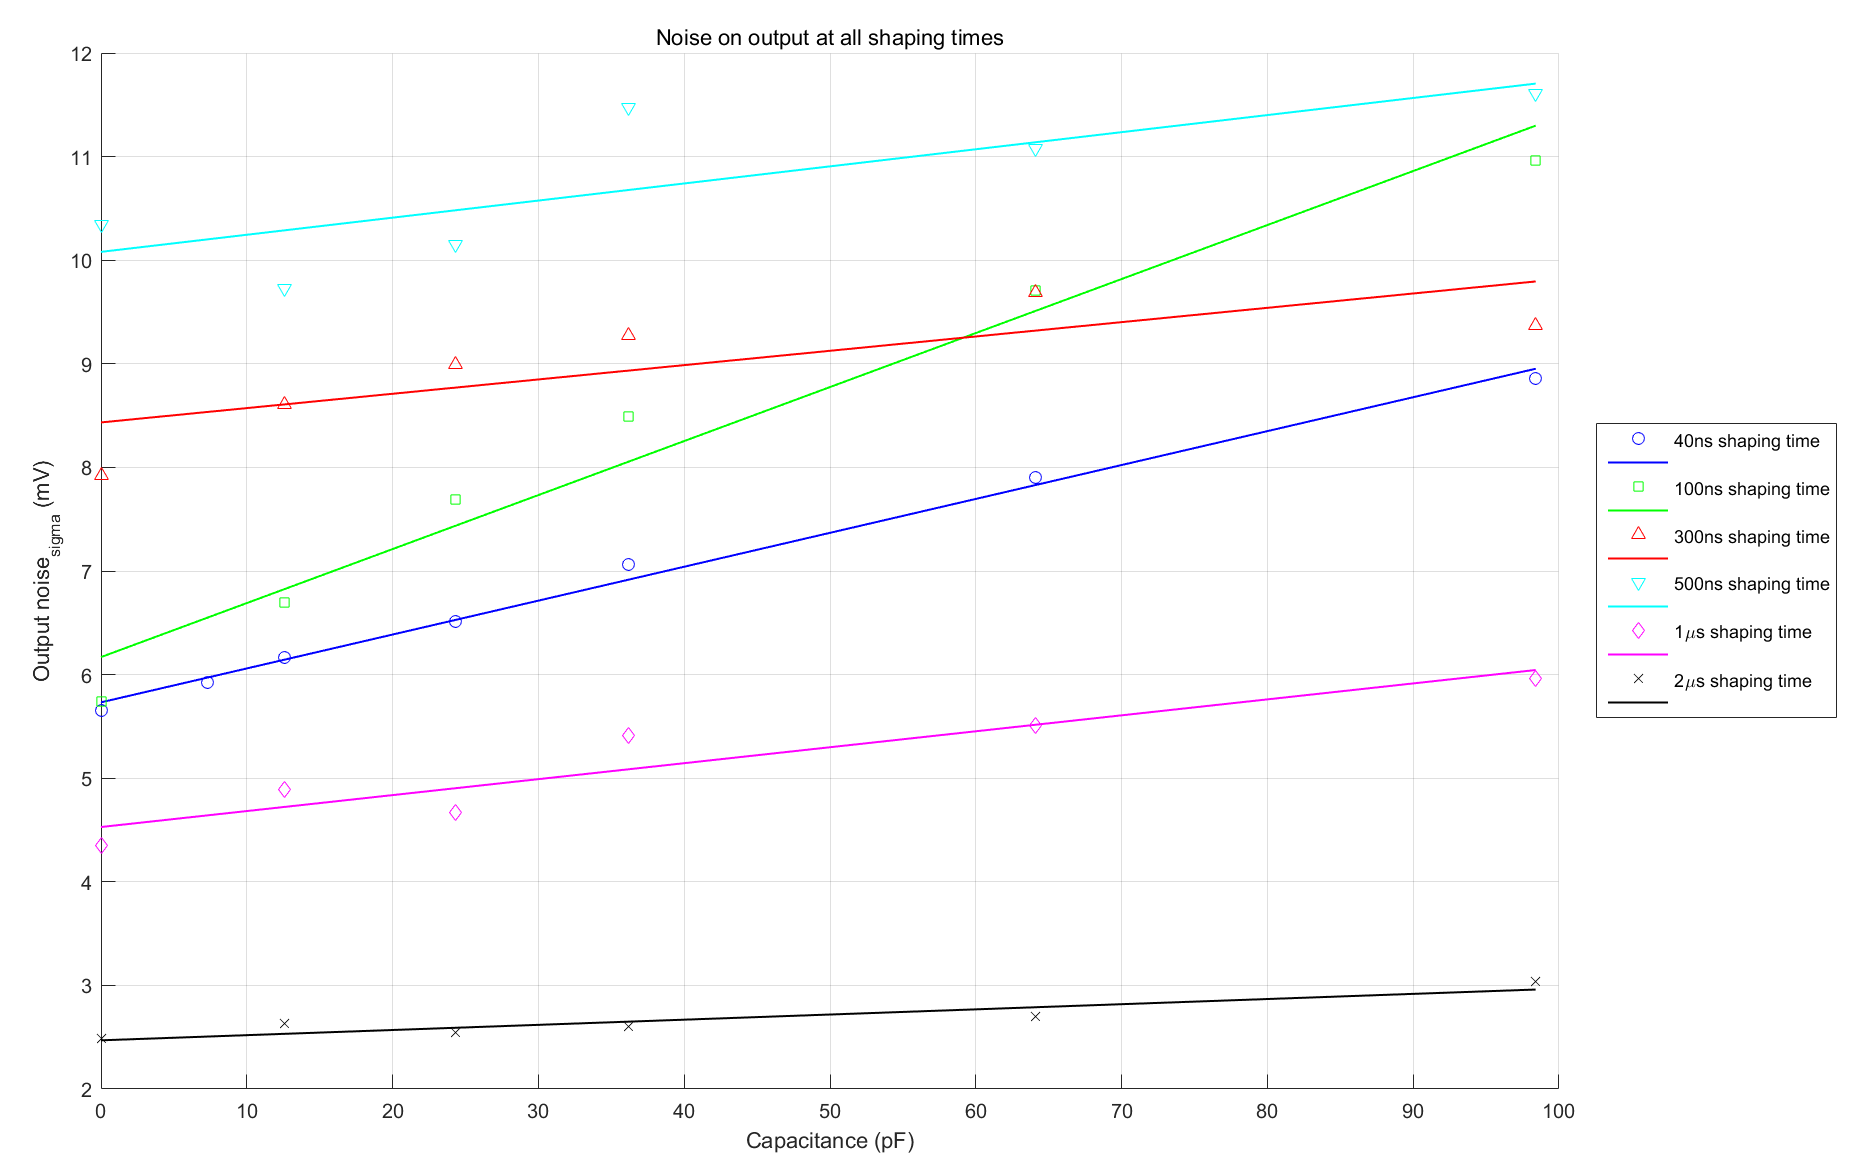
\includegraphics[width=\textwidth]{noise-all-output.png}
	\caption{Measurements of the noise on the IDE1180 output vs. input capacitive load. Calculated with automatic gain compensation.}
	\label{fig-noise-all-output}
\end{figure} 

\begin{figure}[h] %Noise combine
	\centering
	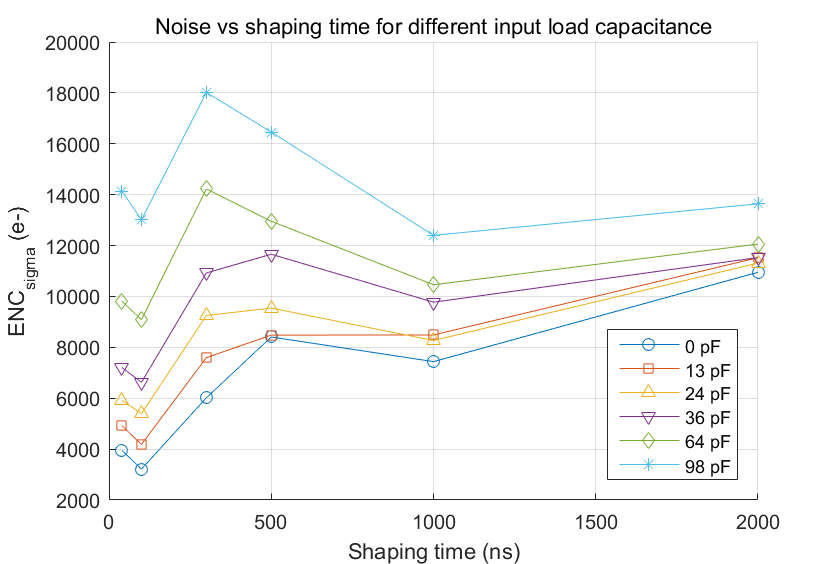
\includegraphics[width=0.7\textwidth]{noise-vs-shape.png}
	\caption{Measurements of the \gls{ENC} vs. shaping time.}
	\label{fig-noise-shape}
\end{figure} 

%\newpage
\newpage
\subsection{Noise from Input Circuitry}
\label{ide-noise-input}

Since the noise measurements in the datasheet were performed directly on the \gls{asic} while the measurements at \gls{uib} are performed on the \gls{PCB}, it is easy to assume that the differences in noise are due to the extra input circuitry on the \gls{PCB}. Therefore, noise measurements were performed with six different connections on the input. This was done with method 1 mentioned at the beginning of section \ref{ide-noise} (except for measurement 6 which is using method 2), with 0 pF input load capacitance. Table \ref{tab-gain-adc} is used for gain compensation. The six connections were as following:
\begin{enumerate}  
	\item No input jumper on SV2 in figure \ref{fig-capmount} (SMA connector and 1pF capacitor disconnected from the \gls{asic}).
	\item Input jumper on SV2 (SMA connector and 1pF connected).
	\item As 2, but aluminium foil covering input SMA.
	\item Input jumper on SV2. SMA-BNC and BNC-LEMO adapters and short LEMO cable connected. Cable left floating.
	\item As 4, but cable connected to wave generator. Generator powered on, but the output is turned off.
	\item As 5, but with a ramp pulse from the generator output.   
\end{enumerate}

\begin{table}[h!]
	\begin{center}
		\caption{Noise measurements with different input circuitry connected.}
		\label{tab-noise-input}
		\begin{tabular}{ccccccc}\toprule
			\textbf{Measurement \#}      & 1    & 2    & 3    & 4    & 5    & 6   \\ 
			\textbf{ENC$_\sigma$ [e-]} & 1642 & 3578 & 3502 & 3527 & 3620 & 3944   \\ \bottomrule
		\end{tabular}
	\end{center}
\end{table}

The main conclusion from table \ref{tab-noise-input} is that the input circuitry has a huge impact on the noise at low capacitance. From measurements 2-5, we see that the adapters, cable, and wave generator do not contribute noticeably to the noise. We also see an increase in noise between measurements 5 and 6, which indicates that method 2 is not a reliable form of measurement. Even though the noise for measurement \#1 in table \ref{tab-noise-input} is much lower, it is still twice the 0 pF measurement in figure \ref{fig-ide-noise}. However, the input of the \gls{asic} is still connected to one of the pins of the pin header, serving as an extra noise source that was not present in the measurement by IDEAS. 

%%XXX figures for method 1 and 2, from noise docx. 2016.05.03. Maybe not



\section{Gain Linearity}
\label{ide-linearity}

Gain linearity has been measured by saving pulses from the Agilent oscilloscope and using Matlab to find the pulse peak value. This was done since the buffer does not cover the entire dynamic range of the IDE1180. The IDE1180 was inside a Faraday cage. Since these measurements are only based on a single pulse for each data point, they have an extra inaccuracy from the noise that would be avoided by saving pulse height histograms on the ADC. 

\begin{figure} %2016.07.18 & 2016.08.12
	\centering
	\begin{subfigure}{.5\textwidth}
		\centering
		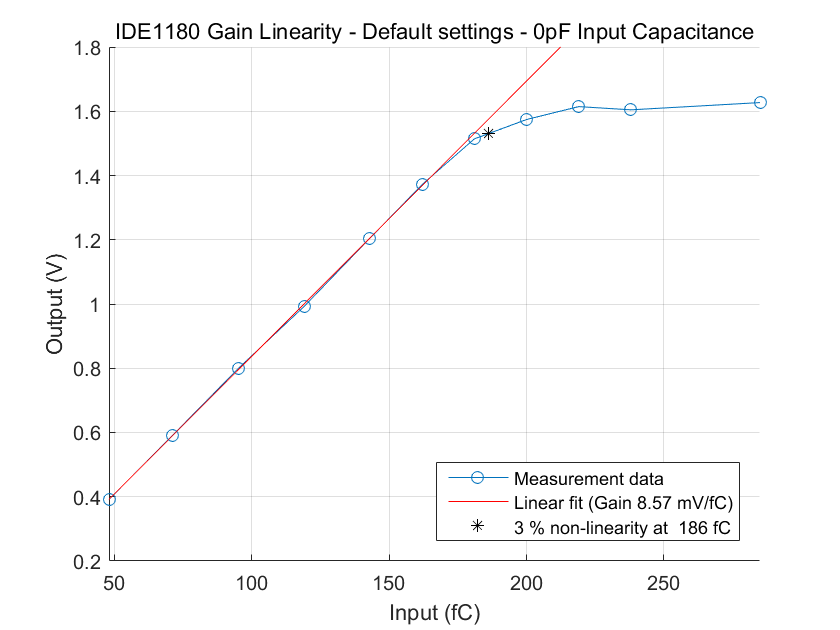
\includegraphics[width=\linewidth]{40ns_0pF.png}
		\caption{40 ns shaping time.}
		\label{fig-gainlin-40n}
	\end{subfigure}%
	\begin{subfigure}{.5\textwidth}
		\centering
		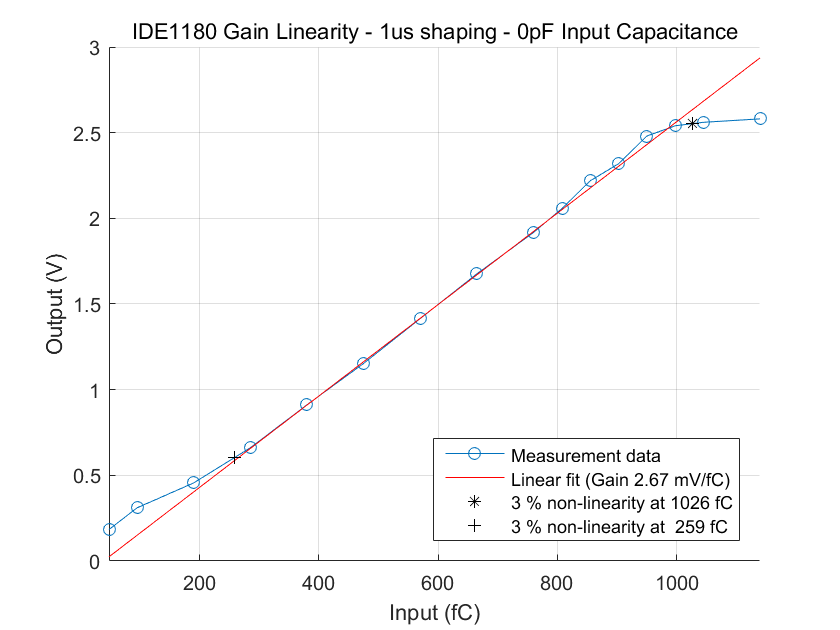
\includegraphics[width=\textwidth]{1us_0pF.png}
		\caption{1 $\mu$s shaping time.}
		\label{fig-gainlin-1u} 
	\end{subfigure}
	\caption{Two examples of gain linearity measurements.}
	\label{fig-gainlin}
\end{figure}

Figure \ref{fig-gainlin} shows two gain linearity graphs. The rest are in appendix \ref{a-gainlin}. The measurements at default settings look very much as expected, but all the other measurements show a bump in the low end, like in figure \ref{fig-gainlin-1u}. The source of this is unknown, but it is likely not from measurement inaccuracies, since the same bump is visible for all the measurements. It is possible that it is somehow related to the pole-zero cancellation that is active for these configurations, but not the default setting. Another possibility is that the bump comes from noise, since the noise has a higher relative effect on weak signals. As seen in figure \ref{fig-noise-shape}, the noise is higher for the other shaping times than for default settings. 

\section{Dynamic Range}
\label{ide-dynamicrange}
%Noise-gain linearity
The dynamic range of the pre-amplifier shaper is on the lower level limited by the noise. To be able to easily discern the signal from noise, the lower end of the dynamic range has been defined as 10 times the noise. The higher end of the dynamic range is set from the gain linearity curves, as the point where the curve is no longer linear. Table \ref{tab-dynrange} shows the low and high limits to the dynamic range from the noise and gain linearity. The low limit from the gain linearity will not necessarily be a problem, but it is still listed in the table so it is not forgotten. It is possible to compensate for it using a linearising circuit or algorithm. 

\begin{table}[h!]
	\begin{center}
		\caption{Dynamic range measurements.}
		\label{tab-dynrange}
		\begin{tabular}{lccc}\toprule
			\textbf{Setting \&}     & \textbf{Low limit [fC]} & \textbf{Low limit [fC]}      & \textbf{High limit [fC]}     \\
			\textbf{input load}    & (noise*10) & (gain linearity) & (gain linearity) \\ \midrule
			40 ns 0 pF     & 6.4     &                & 186            \\
			40 ns 36 pF    & 11.5     &                & 235            \\
			500 ns 0 pF    & 13.4     & 80             & 180            \\
			500 ns 36 pF   & 20.3    & 97             & 211            \\
			1 $\mu$s 0 pF  & 12.0    & 259            & 1026           \\
			1 $\mu$s 36 pF & 15.7     & 355            & 1040           \\
			2 $\mu$s 0 pF  & 17.6    & 553            & 1769           \\
			2 $\mu$s 36 pF & 18.4    & 506            & 1755    \\ \bottomrule
		\end{tabular}
	\end{center}
\end{table}

The dynamic range has only been accurately calculated for the default gain setting. For the other three gain settings, the higher end of the dynamic range has been estimated by observing the output of the IDE1180 using the Tektronix oscilloscope. See table \ref{tab-dynrange-estimate}. The actual maximum input charge is slightly lower than this, as it is hard to see on an oscilloscope exactly when the pulse height increase stops being linear.
%table from gain excel
\begin{table}[h!]
	\begin{center}
		\caption{Dynamic range estimates for different gain settings.}
		\label{tab-dynrange-estimate}
		\begin{tabular}{clc}\toprule
			&\textbf{PA\_GAIN<1:0>} & \textbf{$\mathbf{Q_{in_{max}}}$ [fC]}   \\ \midrule
		    00&GND-GND     & 200   \\
			01&GND-3V3     & 240       \\
			10&3V3-GND     & 300    \\
			11&3V3-3V3     & 440   \\ \bottomrule
		\end{tabular}
	\end{center}
\end{table}

\subsection{Input Sharing}
\label{ide-inputshare}

Input sharing was investigated as a method to increase the dynamic range to a higher level than what is possible by reducing the gain. The thought behind this was to connect multiple channels of the IDE1180 to the same signal, expecting that the signal charge would spread evenly across the channels. From this, it would be possible to divide the signal by a number between 2 and 15. However, tests showed that the charge was not spread evenly across the channels, making this method unreliable. 

%It was however discovered that it was reliable if the outputs of all the used channels are connected together. Table \ref{tab-input-share} shows the estimated gain and dynamic range of the complete system with different amounts of channels connected.This was done using the Agilent oscilloscope with different amounts of channels connected, and the IDE1180 inside a Faraday cage. One channel is only with channel one connected, two channels is channel one and two, etc. Figure \ref{fig-input-sharing} shows that the dynamic range is linearly increased using this method.

%\begin{table}[h!]
%	\begin{center}
%		\caption{Input sharing gain and dynamic range estimates.}
%		\label{tab-input-share}
%		\begin{tabular}{ccccc}\toprule
%			\textbf{Channels} & \textbf{Output voltage at} & \textbf{Gain}     & \textbf{Saturation} & \textbf{Output voltage} \\
%			& \textbf{190 fC input [mV]} & \textbf{[mV/fC]} & \textbf{charge [fC]} & \textbf{at saturation [mV]} \\\midrule
%			1          & 1560                             & 8.21 & 190                  & 1560                            \\
%			2          & 1060                             & 5.58 &                      &                                 \\
%			3          & 930                              & 4.89 &                      &                                 \\
%			4          & 810                              & 4.26 & 710                  & 2400                            \\
%			5          & 700                              & 3.68 &                      &                                 \\
%			6          & 610                              & 3.21 &                      &                                 \\
%			7          & 540                              & 2.84 &                      &                                 \\
%			8          & 480                              & 2.53 & 1430                 & 2950                            \\
%			9          & 440                              & 2.32 &                      &                                 \\
%			10         & 400                              & 2.11 &                      &                                 \\
%			11         & 360                              & 1.89 &                      &                                 \\
%			12         & 330                              & 1.74 & 2190                 & 3250                            \\
%			13         & 310                              & 1.63 &                      &                                 \\
%			14         & 280                              & 1.47 &                      &                                 \\
%			15         & 270                              & 1.42 &                      &                                 \\
%			16         & 260                              & 1.36 & 2950                 & 3000                              \\ \bottomrule
%		\end{tabular}
%	\end{center}
%\end{table}
%
%\begin{figure}[h]
%	\centering
%	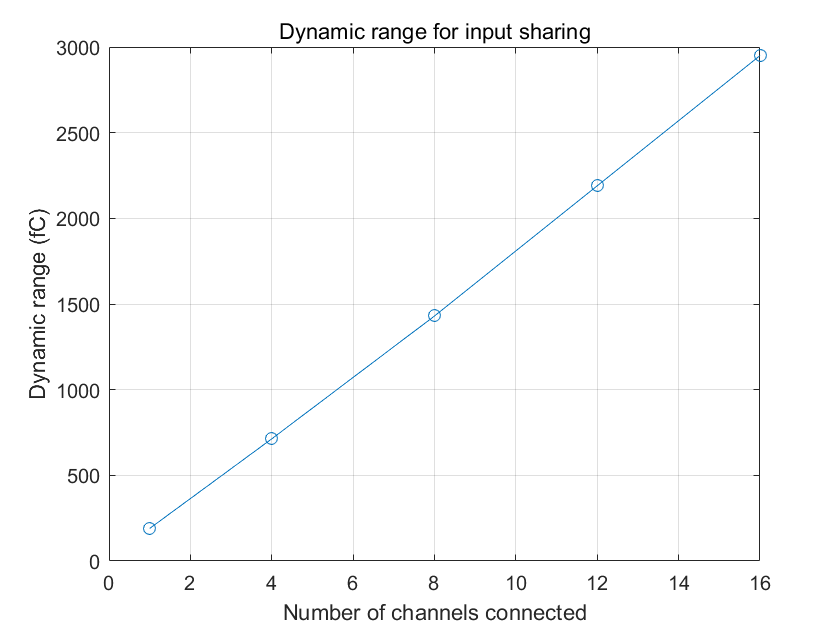
\includegraphics[width=0.7\textwidth]{input-sharing.png}
%	\caption{Dynamic range variations from input sharing.}
%	\label{fig-input-sharing}
%\end{figure} 


\section{Shaping Time}
\label{ide-shapingtime}
%shaping time vs input charge (from gain linearity)
%shaping time vs. C (from gain/risetime/area)

The shaping time has some variations from the input load capacitance and input capacitance. The shaping times listed in table \ref{tab-ide-shaping} are therefore not always accurate. Table \ref{tab-ide-shaping-c} shows shaping time versus input load capacitance, calculated from the data that was used to create figures \ref{fig-IDE1180-shaperamp} to \ref{fig-IDE1180-shaperrisetime}. These fluctuations appear very small and random, and could come from the noise. Figure \ref{fig-shape-example} and appendix \ref{a-shape} show shaping time variations with input charge. These variations are larger, and appear more structured, with a general trend of increased shaping time with higher input charge. These data are calculated from the results of the gain linearity measurements. All the data in this section is calculated from snapshots of a single pulse, and therefore not the most accurate. If accurate measurements of the shaping time is needed, this could be done with a more complex LabVIEW program that calculates the shaping time of every pulse. The difference between the shaping times in table \ref{tab-ide-shaping-c} and figure \ref{fig-shape-40-0-} is caused by the same issue as discussed in section \ref{ide-gain} and figure \ref{fig-box-pulse}. The results in this section can therefore be expected to be slightly higher than what would be obtained with a lower line capacitance. 

\begin{table}[h!]
	\begin{center}
		\caption{Shaping time vs. input load capacitance.}
		\label{tab-ide-shaping-c}
		\begin{tabular}{lccccccc}\toprule
			\textbf{Capacitance [pF]}      & 0    & 7.3    & 12.6    & 24.3    & 36.2    & 64.1 & 90.4   \\ 
			\textbf{Shaping time [ns]} & 63.0 & 63.5 & 59.5 & 60.0 & 62.0 & 53.5 & 61.0   \\ \bottomrule
		\end{tabular}
	\end{center}
\end{table}

\begin{figure} [h!]%2016.07.18 & 2016.08.12
	\centering
	\begin{subfigure}{.5\textwidth}
		\centering
		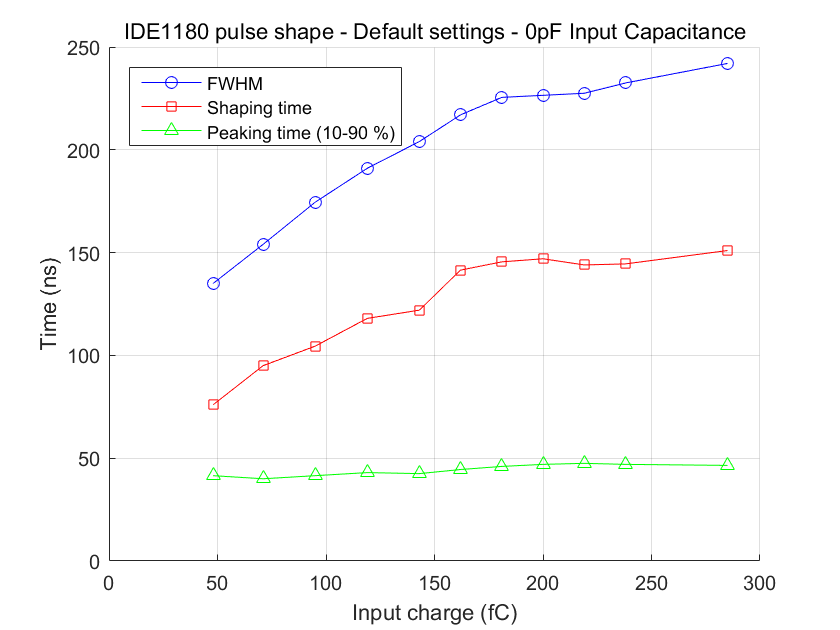
\includegraphics[width=\linewidth]{sh_40_0.png}
		\caption{Default settings.}
		\label{fig-shape-40-0-}
	\end{subfigure}%
	\begin{subfigure}{.5\textwidth}
		\centering
		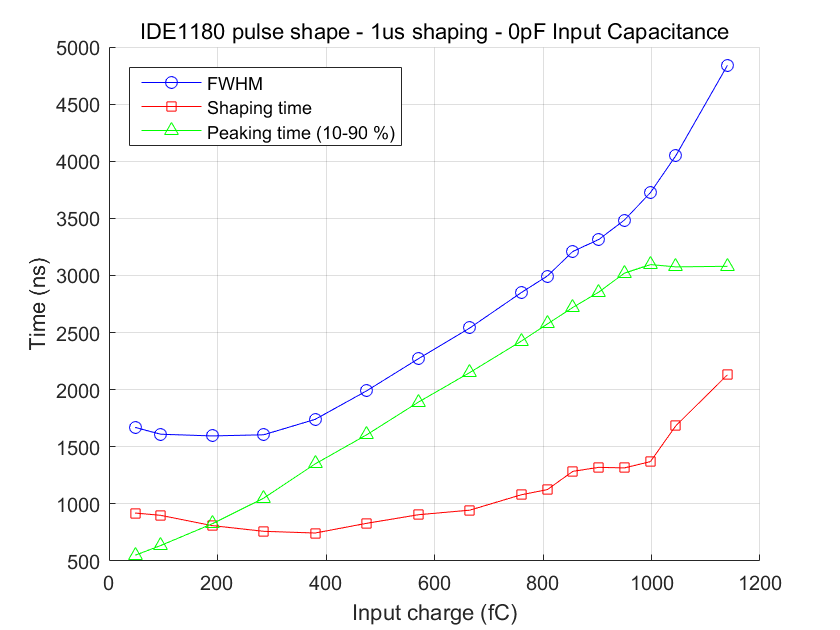
\includegraphics[width=\textwidth]{sh_1_0.png}
		\caption{1 $\mu$s shaping time.}
		\label{fig-shape-1-0-} 
	\end{subfigure}
	\caption{Two examples of shaping time, \gls{FWHM}, and peaking time measurements.}
	\label{fig-shape-example}
\end{figure}

\section{Peaking Time}
\label{ide-risetime}
%from gain linearity measurements

\begin{figure}
	\centering
	\begin{subfigure}{.5\textwidth}
		\centering
		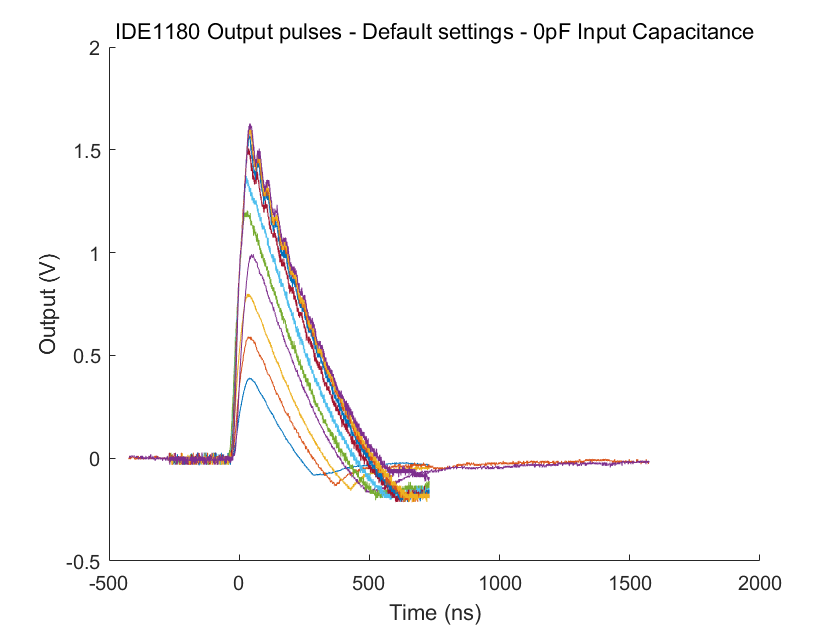
\includegraphics[width=\linewidth]{risetime-default.png}
		\caption{Default settings.}
		\label{fig-IDE1180-risetime-def}
	\end{subfigure}%
	\begin{subfigure}{.5\textwidth}
		\centering
		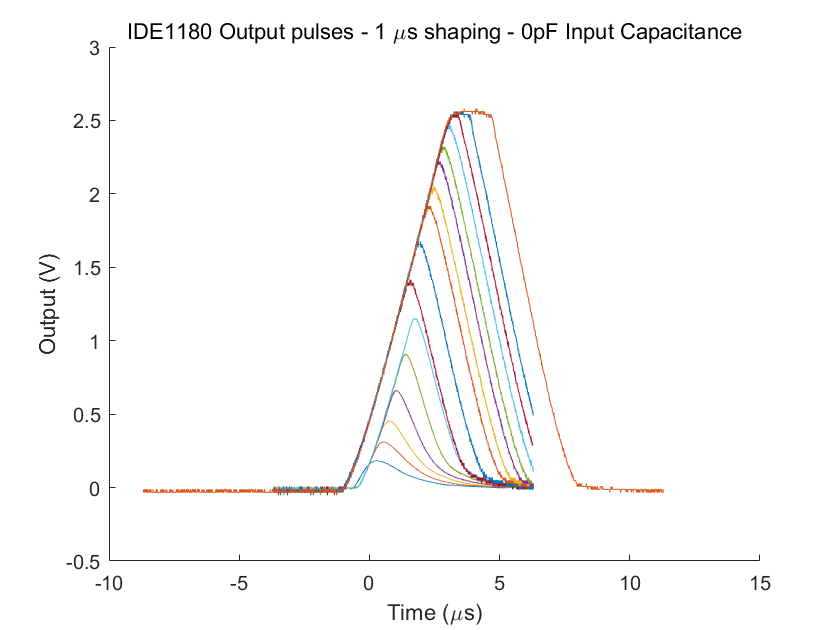
\includegraphics[width=\textwidth]{risetime-1us.png}
		\caption{1 $\mu$s shaping.}
		\label{fig-IDE1180-risetime-1us} 
	\end{subfigure}
	\caption{Output pulses from IDE1180 with input signals of varying charge. These are the pulses used to find gain linearity.}
	\label{fig-IDE1180-risetime}
\end{figure}

%slew rate
Figure \ref{fig-IDE1180-risetime-def} shows that at 40 ns shaping time the slope increases when the amplitude increases, which makes sure that the peaking time is more or less unchanged, see figure \ref{fig-shape-40-0-}. For increased shaping time however, the slope in \ref{fig-IDE1180-risetime-1us} is constant for all input charges. This leads to a greatly increased peaking time for higher input charges, see figure \ref{fig-shape-1-0-}. This unchanging slope looks very linear, which leads to the assumption that this could due to a slew rate limitations. The changes to the system performed to increase the shaping time might have reduced the maximum slew rate, which makes the system unable to increase the voltage fast enough. All peaking time measurements can be seen in appendix \ref{a-shape}.


\section{Crosstalk}
\label{ide-crosstalk}
%http://www.slideshare.net/RohdeSchwarzNA/crosstalk-measurements-for-signal-integrity-applications

It was attempted to measure crosstalk between the channels by measuring the noise on channel 2, with an input signal on channel 1. However, the crosstalk signal was too close to the noise to be noticeable on the noise histogram. Therefore, measurements were instead done by measuring the amplitude of the crosstalk signal by using an external trigger signal from the wave generator. Crosstalk was measured with the ADC, for default and 1 $\mu$s shaping time, see table \ref{tab-crosstalk-adc}. For each shaping time, it was measured for the minimum amplitude from the Tektronix AFG3252 wave generator, and for the maximum amplitude before the in-house buffer cuts the signal. The wave generator signal was sent to channel 1, while the other channels were measured. The crosstalk was also roughly measured for default shaping time using cursors on the Agilent MSO-X 3104A oscilloscope, table \ref{tab-crosstalk-osc}, which showed that the crosstalk is roughly the same three channels away from the signal, as fifteen channels away. Therefore, the ADC measurements, which take some time, were not done for channels 6 to 15. 

\begin{table}[h!]
	\begin{center}
		\caption{Crosstalk estimates using oscilloscope. Input signal to channel 1.}
		\label{tab-crosstalk-osc}
		\begin{tabular}{crlrlrl} \toprule
			\textbf{Channel \#} & \textbf{$\mathbf{V_o}$ [mV]} &\textbf{[\%]}& \textbf{$\mathbf{V_o}$ [mV]} & \textbf{[\%]}& \textbf{$\mathbf{V_o}$ [mV]} &\textbf{[\%]}\\
			     & ($Q_{in}=48 fC$) && ($Q_{in}=95 fC$) && ($Q_{in}=190 fC$)& \\ \midrule
			1  & 375  & 100 \% & 775 & 100 \% & 1500 & 100 \% \\
			2  & 6.5 & 1.73 \%   & 10  & 1.29 \%   & 18   & 1.20 \%   \\
			3  & 5.5 & 1.47 \%   & 8.5 & 1.10 \%   & 14   & 0.93 \%   \\
			4  & 4.5 & 1.20 \%   & 6   & 0.77 \%   & 8    & 0.53 \%   \\
			5  & 4.5 & 1.20 \%   & 6   & 0.77 \%   & 8    & 0.53 \%   \\
			6  & 4 & 1.07 \%   & 6   & 0.77 \%   & 8    & 0.53 \%   \\
			7  & 4 & 1.07 \%   & 6   & 0.77 \%   & 8    & 0.53 \%   \\
			8  & 4 & 1.07 \%   & 6   & 0.77 \%   & 8    & 0.53 \%   \\
			9  & 4 & 1.07 \%   & 6   & 0.77 \%   & 8    & 0.53 \%   \\
			10 & 4 & 1.07 \%   & 6   & 0.77 \%   & 8    & 0.53 \%   \\
			11 & 4 & 1.07 \%   & 6   & 0.77 \%   & 8    & 0.53 \%   \\
			12 & 4 & 1.07 \%   & 6   & 0.77 \%   & 8    & 0.53 \%   \\
			13 & 4 & 1.07 \%   & 6   & 0.77 \%   & 8    & 0.53 \%   \\
			14 & 4 & 1.07 \%   & 6   & 0.77 \%   & 8    & 0.53 \%   \\
			15 & 4 & 1.07 \%   & 6   & 0.77 \%   & 8    & 0.53 \%   \\
			16 & 4 & 1.07 \%   & 6   & 0.77 \%   & 8    & 0.53 \%      \\ \bottomrule
		\end{tabular}
	\end{center}
\end{table}

The noise during the table \ref{tab-crosstalk-osc} was estimated to 4 mV, so the highest crosstalk was about 4.5 times the noise. Relative to the signal on channel 1, the crosstalk was between 0.5 \% and 1.75 \% of the signal strength. 

\begin{table}[h!]
	\begin{center}
		\caption{Crosstalk measurements. Input signal to channel 1.}
		\label{tab-crosstalk-adc}
		\begin{tabular}{ccccc} \toprule
			\textbf{Channel \#} & \textbf{$\mathbf{V_o}$ [mV]} & \textbf{$\mathbf{V_o}$ [mV]} & \textbf{$\mathbf{V_o}$ [mV]} & \textbf{$\mathbf{V_o}$ [mV]} \\
			& ($Q_{in}=48 fC$) & ($Q_{in}=95 fC$) & ($Q_{in}=48 fC$)  & ($Q_{in}=475 fC$)\\ 
			& (40 ns shaping)& (40 ns shaping)& (1 $\mu$s shaping)& (1 $\mu$s shaping) \\ \midrule
			1       & 411.6 (100 \%) & 839.3 (100 \%)   & 157.2 (100 \%) & 990.8 (100 \%) \\
			2       & 6.5 (1.58 \%)    & 10.8 (1.29 \%)    & 3.2 (2.04 \%)   & 10.8 (1.09 \%)  \\
			3       & 5.6 (1.36 \%)    & 8.0 (0.95 \%)     & 3.4 (2.16 \%)   & 10.8 (1.09 \%)  \\
			4       & 4.9 (1.19 \%)    & 5.3 (0.63 \%)     &       & 3.1 (0.31 \%)   \\
			5       & 4.9 (1.19 \%)    & 5.4 (0.64 \%)     &       &       \\
			16      & 5.2 (1.26 \%)    & 5.4 (0.64 \%)     & 2.3 (1.46 \%)   & 2.9 (0.29 \%) \\ \bottomrule
		\end{tabular}
	\end{center}
\end{table}

Table \ref{tab-crosstalk-adc} shows crosstalk between 0.3 \% and 2 \% of the signal strength. The noise was measured to roughly 3 mV for these measurements, making the highest crosstalk 3.6 times the noise. These measurements are a lot more accurate than the estimates in table \ref{tab-crosstalk-osc}, but the estimates are also included in this thesis as they cover the high end of the dynamic range that cannot currently be measured using the ADC. 

\section{Power Consumption}
\label{ide-power}

Power consumption was measured for different shaping times by connecting an ampere-meter between the power supply and the IDE1180. The power consumption was not affected by the input charge to the chip. 

\begin{table}[h!]
	\begin{center}
		\caption{Power consumption measurements.}
		\label{tab-ide-power}
		\begin{tabular}{ccccc}\toprule
			\textbf{Shaping time [ns]}      & 40 (Default)    & 500    & 1000    & 2000       \\ 
			\textbf{Power consumption [mW]} & 224 & 235 & 223 & 208    \\ \bottomrule
		\end{tabular}
	\end{center}
\end{table}

The power consumption values in table \ref{tab-ide-power} are a lot higher than the 32 mW from the datasheet. This is expected, as the datasheet is made from measurements directly on the chip. The extra power consumption comes from components on the PCB. 

\section{Pile-up}
\label{ide-pileup}

The maximum count rate that can be used without causing pile-up has been calculated from the time between the pulse starts to rise until the undershoot has stabilized. This has been measured at the highest input signal of the dynamic range, as the pulse width is slightly increased by input charge. C depancy?XXX

XXX table

\comm{
\section{Resolution}
\label{ide-resolution}
%%ADC+noise
The resolution of the system is mainly limited by the noise and the \gls{ADC}. 
}

\section{The 7048 Evaluation Board}
\label{ide-7048}

As mentioned in the beginning of this chapter, two evaluation boards were received by IDEAS. The gain on the 7048 board was briefly tested, shown in table \ref{tab-gain-adc-7048}. The difference between this and and the 7045 board, table \ref{tab-gain-adc}, led to an investigation on the gain settings of the 7048 board. This, in table \ref{tab-gains-7048}, shows that on the 7048 chip, unlike the 7045, the gain was different for gain inputs floating and to ground. It should also be noted that for the 7045 board, gain inputs to ground gives the highest gain, while on the 7048 board 3.3~V gives the highest gain. Because of this strange behaviour, the 7048 board has not been tested any more, as it is hard to trust its settings. 
%In table \ref{tab-gains-7048} "0" is right jumper position, "1" is left position, and "X" is no jumper in place.

\begin{table}[h!]
	\begin{center}
		\caption{Gain [mV/fC] vs. capacitance measured with ADC on the 7048 PCB, with no jumpers in place.}
		\label{tab-gain-adc-7048}
		\begin{tabular}{cccccc}\toprule
			\textbf{PA\_GAIN<1:0>} & \textbf{0pF}  & \textbf{10pF} & \textbf{56pF} & \textbf{56pF} & \textbf{100pF} \\ \midrule
			X-X     & 3.19 & 2.66  & 2.23  & 1.51 & 1.12   \\ \bottomrule
		\end{tabular}
	\end{center}
\end{table}

\begin{table}[h!]	%%XXXfix 00 11 here
	\begin{center}
		\caption{Gain [mV/fC] measurements for different gain settings measured with oscilloscope on the 7048 evaluation board.}
		\label{tab-gains-7048}
		\begin{tabular}{clc}\toprule
			&\textbf{PA\_GAIN<1:0>} & \textbf{Gain}   \\ \midrule
			11&3V3-3V3 & 5.4  \\
			1X&3V3-X & 5.2  \\
			10&3V3-GND & 3.45 \\
			X1&X-3V3 & 5.3  \\
			XX&X-X & 3.2  \\
			X0&X-GND & 2.35 \\
			01&GND-3V3 & 2.2  \\
			0X&GND-X& 1.8  \\
			00&GND-GND & 1.0   \\ \bottomrule
		\end{tabular}
	\end{center}
\end{table}


\end{document}